\chapter{A 2-step evolution model driven by digital elastica minimization}
\chaptermark{A 2-step evolution model}
\label{chapter:flip-flow}

In the previous chapter we have presented a local combinatorial model using multigrid convergent estimator that proved to be very successful in optimizing the digital elastica but too slow to be used in practice. We have also attempted to derive a global optimization model, but unfortunately such model is unlikely to be solved in the current state of art of binary optimization techniques. In this chapter we present a second local optimization model that is much faster than~\cref{ch5:alg:local-search} but with fewer guarantees of optimality.

\daniel{
We describe the binary non-submodular FlipFlow energy and discuss some curious aspects of it in~\cref{ch6:sec:flipflow-model}. Optimization strategies are presented in~\cref{ch6:sec:optimization-method,ch6:sec:evaluation-across-rings}. Finally, we describe an application of the FlipFlow model to image segmentation in~\cref{ch6:sec:data-term-image-segmentation}.
}


\section{FlipFlow model}
\label{ch6:sec:flipflow-model}

In this section we describe the FlipFlow model that aims to evolve an initial digital shape $\Ds$ into another of lower digital elastica value. The FlipFlow algorithm consists into deciding, at each iteration $k$, which pixels in the \emph{inner boundary} of $\Ds^{(k)}$ are to be removed  and which are to be kept. 

\subsection{Definitions}
\label{ch6:subsec:definitions}

Let $\Ds$ be a digital shape with domain $\Omega \subset \mathbb{Z}^2$. We describe a flow $\left \{ \Ds^{(k)} \; | \; k \geq 0, \Ds^{0} = \Ds \right\}$ intended to decrease the digital elastica energy of $\Ds$.

We assume an ordering in $\Omega$, i.e., there exists a bijective function $\omega : \Omega \rightarrow \{1 \cdots |\Omega| \}$. Moreover, let $X_{\omega}:\Omega \rightarrow 2^{\{0,1\}}$ be an operator that transforms digital sets in its corresponding set of binary variables, i.e.,
\begin{align*}
	X_{\omega}(\Omega) := \left\{ x_{\omega(p)} \in \{0,1\} \; | \; p \in \Omega \right\}.
\end{align*}
%
We will simply write $X(\Omega)$, assuming that exists an underlying ordering function $\omega$.

A $\{0,1\}$ assignment of the variables in $X(\Omega)$ is denoted $x(\Omega)$. We define the sum of a digital set $\Ds$ and an assignment $x(\Omega)$ as
\begin{align*}
	\Ds + x(\Omega) = \Ds \cup \left\{ p \; | \; p \in P, x_{\omega(p)}=1 \right\}.
\end{align*}
%
Next, we define the set of optimization variables. In order to guarantee connectivity and thus avoid the enforcement of the topological constraints discussed in~\cref{ch5:subsec:topological-constraints}, we limit the optimization region to a subset of $\Omega$, namely the inner pixel boundary of  $\Ds^{(k)}$. \daniel{We recall the definition given in~\cref{chapter:digital-elastica}}.
\begin{align*}
	I(\Ds) := \left\{ \: p \; | \; p \in \Ds, |\mathcal{N}_4(x) \cap \Ds|<4 \: \right\},
\end{align*}
%
%Further, we write $\overline{I}(\Ds)$ to denote the inner pixel boundary of the complement of $\Ds$, i.e., $\overline{I}(\Ds) := I(\overline{\Ds})$.
%
To simplify notation, the inner pixel boundary of $\Ds^{(k)}$ is simply denoted $I^{(k)}$. At each iteration, the set $X^{(k)}$ of optimization variables is defined as
\begin{align*}
	X^{(k)} := X(I^{(k)}).
\end{align*}
%
In the case we optimize the complement of $\Ds$, we write $\overline{X}^{(k)}$, i.e., $\overline{X}^{(k)} = X(I(\overline{\Ds}^ {(k)}))$.

An assignment of $X^{(k)}$ is simply denoted $x^{(k)}$. 


\subsection{\daniel{Model and algorithm}}
\label{ch6:subsec:algorithm}

We recall the definition of the II digital curvature estimator \daniel{(see~\cref{ch4:sec:geometric-measurements} for details):}
\begin{align}
	\hat{\kappa}^2(p) &= c_1\Big( c_2 - | B_r(p) \cap \Ds^{(k)} | \Big)^2, 
	\label{eq:curvature-estimator-pixels}
\end{align}
where $c_1=3/r^6$ and $c_2=\pi r^2/2$. 
%
The following sets are important in the expansion of $~\cref{eq:curvature-estimator-pixels}$.
\begin{align*}
	\begin{array}{rll}
	F^{(k)} &:= \Ds^{(k)} \setminus I^{(k)} & \text{ \daniel{(Sure foreground) }} \\
	F_r^{(k)}(p) &:= F^{(k)} \cap B_r(p) &\\
	I_r^{(k)}(p) &:= I^{(k)} \cap B_r(p) & \\
	X_r^{(k)}(p) &:= X\big( I_r^{(k)}(p) \big). & \\	
	\end{array}
\end{align*}
%
%
Expanding~\cref{eq:curvature-estimator-pixels}, we get 
\begin{align}
  \hat{\kappa}^2(p) &= c_1\Big( c_2 - |F_{r}^{(k)}(p)| - \sum_{x_j \in X_r^{(k)}(p)} {x_j} \Big)^2 \nonumber \\
   &= c_1 \Big( C + 2\left( |F_{r}^{(k)}(p)| - c_2 \right) \hspace{-2mm}\sum_{x_j \in X_{r}^{(k)}(p)}\hspace{-2mm}{x_j} + \hspace{-2mm}\sum_{x_j \in X_{r}^{(k)}(p)}\hspace{-2mm}{x_j^2} + \hspace{-2mm}\sum_{ \substack{x_j,x_l \in X_{r}^{(k)}(p) \\ j<l} }\hspace{-2mm}{2x_jx_l}  \Big),
   \label{eq:digital-squared-curvature-term}
\end{align}
where $C=c_2^2 - 2c_2 \cdot |F_{r}^{(k)}(p)| + |F_{r}^{(k)}(p)|^2$ is a constant. As~\cref{eq:digital-squared-curvature-term} is a term to be optimized, we can ignore constants and multiplication factors. Moreover, as we are in a binary optimization setting, we can  further simplify~\cref{eq:digital-squared-curvature-term} by exploiting the binary character of variables and eliminating monomials of second order. We define the following family
of energies for given parameters $\vec{\theta}=(\alpha,\beta ) \geq 0$ \daniel{and $m \geq 0$}
\begin{align}
  E_{(\vec{\theta},m)}^{flip}(\Ds^{(k)},X^{(k)}) =& \sum_{x_j \in X^{(k)}}{\alpha s(x_j)} + \nonumber \\ 
  & \sum_{ \substack{p \in \\ \daniel{R_m(\Ds^{(k)})}}}{ 2c_1 \beta  \Big( { (1/2+ |F_{r}^{(k)}(p)|-c_2) \cdot \sum_{ \substack{ x_j \in \\ X_{r}^{(k)}(p)}}{x_j} } + \sum_{ \substack{j<l, \\ x_j,x_l \in \\ X_{r}^{(k)}(p) } }{x_jx_l} \Big) },
  \label{eq:energy-family}
\end{align}
where $s(\cdot)$ denotes the length penalization term, written as
\begin{align}
  s(x_{w(p)})=\sum_{q \in \mathcal{N}_4(p)}{ t(q) }, \quad \text{where } t(q) = \left\{\begin{array}{ll}
  (x_{w(p)}-x_{w(q)})^2, & \text{if } q \in I^{(k)}\\
  (x_{w(p)}-1)^2, & \text{if } q \in F^{(k)}\\
  (x_{w(p)}-0)^2, & \text{otherwise. }
  \end{array}\right.
  \label{eq:length-penalization}
\end{align}
%
%
We recall that $R_m$ refers to the $m$-ring defined in~\cref{ch5:sec:local-combinatorial-scheme}. Each choice of $m$ generates a different flow, which is generally described in the \emph{FlipFlow}~\cref{ch6:alg:evolution-model}. To optimize~\cref{eq:energy-family} we use the QPBOI algorithm \cite{rother07qpbo}.


\begin{algorithm}
 \SetKwData{It}{k}
 \SetKwData{MIt}{maxIt}
 \SetKwData{Delta}{delta}
 \SetKwInOut{Input}{input}\SetKwInOut{Output}{output}
 \SetKwComment{comment}{//}{}
 
 \Input{A digital set $\Ds$; The ring number $m$; Length($\alpha$), curvature($\beta$) grouped in parameter vector $\vec{\theta}$; the maximum number of iterations \MIt;}
 \BlankLine
 $\Ds^{(0)} \longleftarrow \Ds$\;
 $k \longleftarrow 1$\;
 \While{ \It $<$ \MIt  }{ 	
	\comment{Shrink mode}
	\If{ \It is even }{	 
	 	$x^{(k-1)} \longleftarrow \displaystyle \argmin_{X^{(k-1)}} E_{(\vec{\theta},m)}^{flip}(\Ds^{(k-1)},1-X^{(k-1)})$\; 	
 		$\Ds^{(k)} \longleftarrow F^{(k-1)} + x^{(k-1)}$\;
 	}
	\comment{Expansion mode} 	
 	\Else{	
	 	$\overline{x}^{(k-1)} \longleftarrow \displaystyle \argmin_{\overline{X}^{(k-1)}} E_{(\vec{\theta},m)}^{flip}(\Ds^{(k-1)},1-\overline{X}^{(k-1)})$\;
 		$\Ds^{(k)} \longleftarrow \overline{ \overline{F}^{(k-1)} + \overline{x}^{(k-1)}}$\; 	
 	}
 	
	\It $\longleftarrow$ \It $+1$\;
	
 }
 \caption{FlipFlow algorithm.}
 \label{ch6:alg:evolution-model}  
\end{algorithm}

\subsection{Algorithm discussion}
\label{ch6:subsec:flipflow-algorithm-discussion}

\begin{figure}
\begin{minipage}{0.49\textwidth}
\center
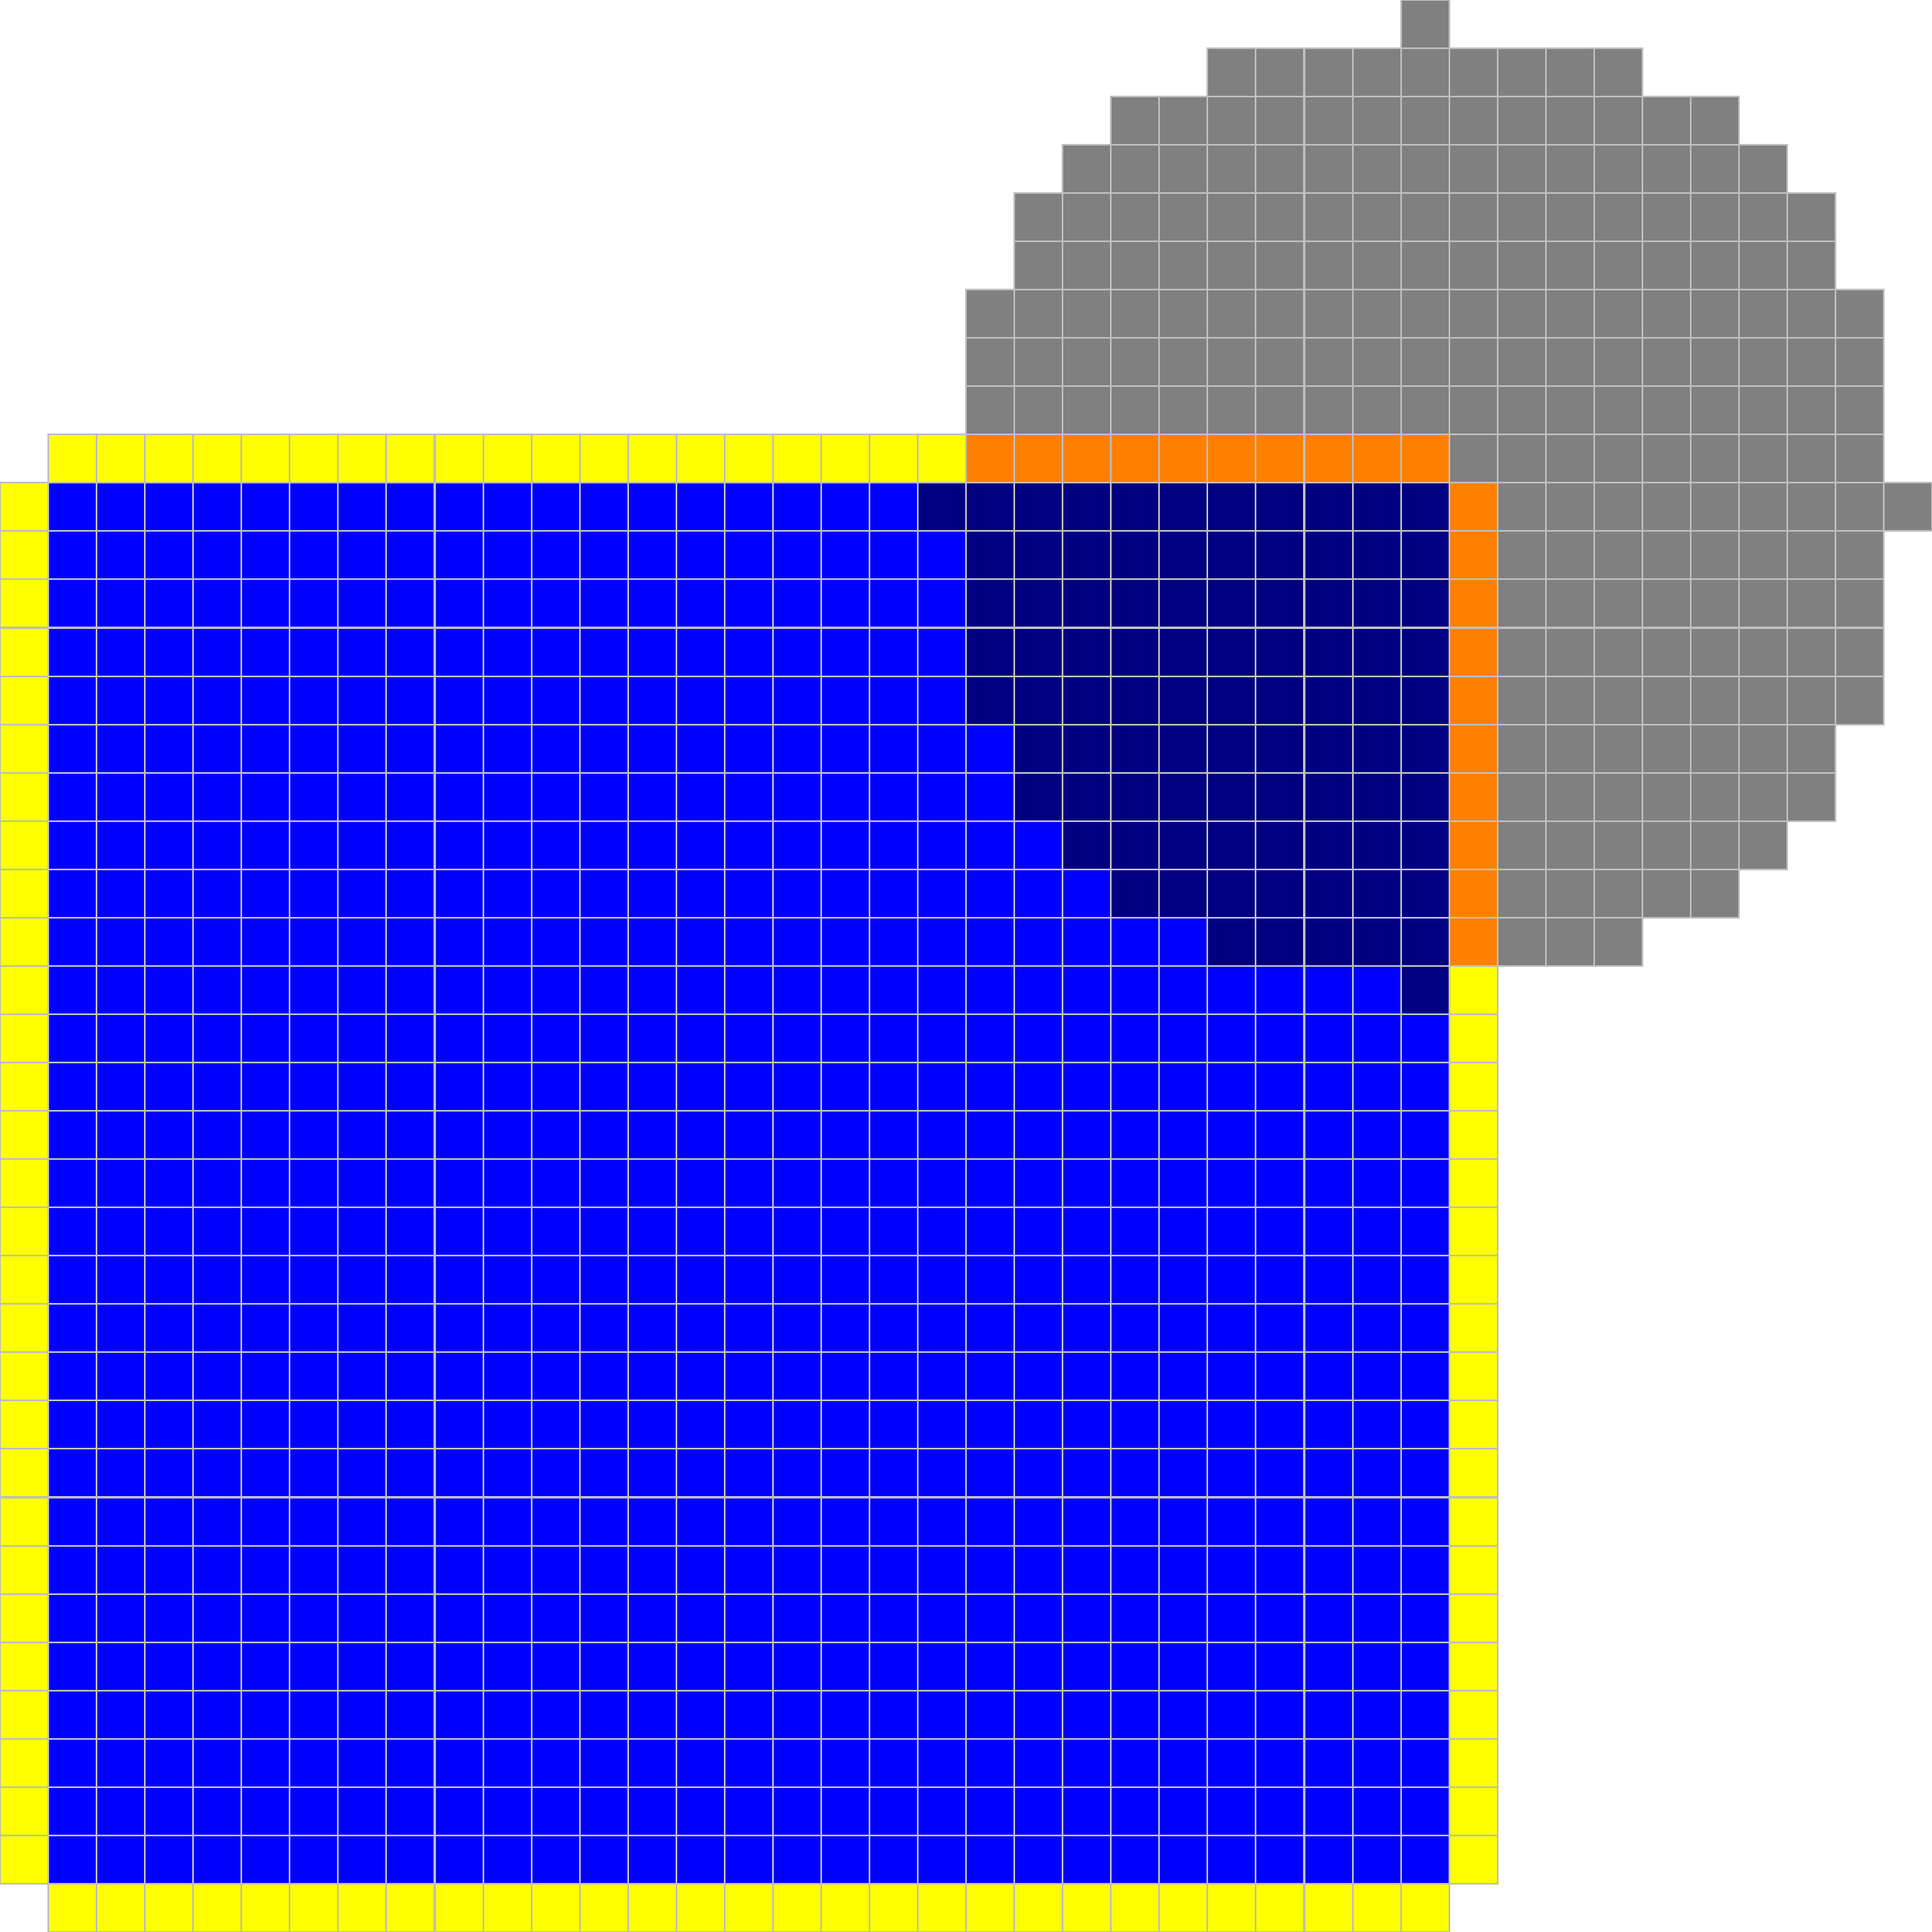
\includegraphics[scale=0.15]{figures/chapter6/contour-information/before-opt.pdf}
\label{ch6:fig:contour-info-1}
\end{minipage}%
\begin{minipage}{0.49\textwidth}
\center
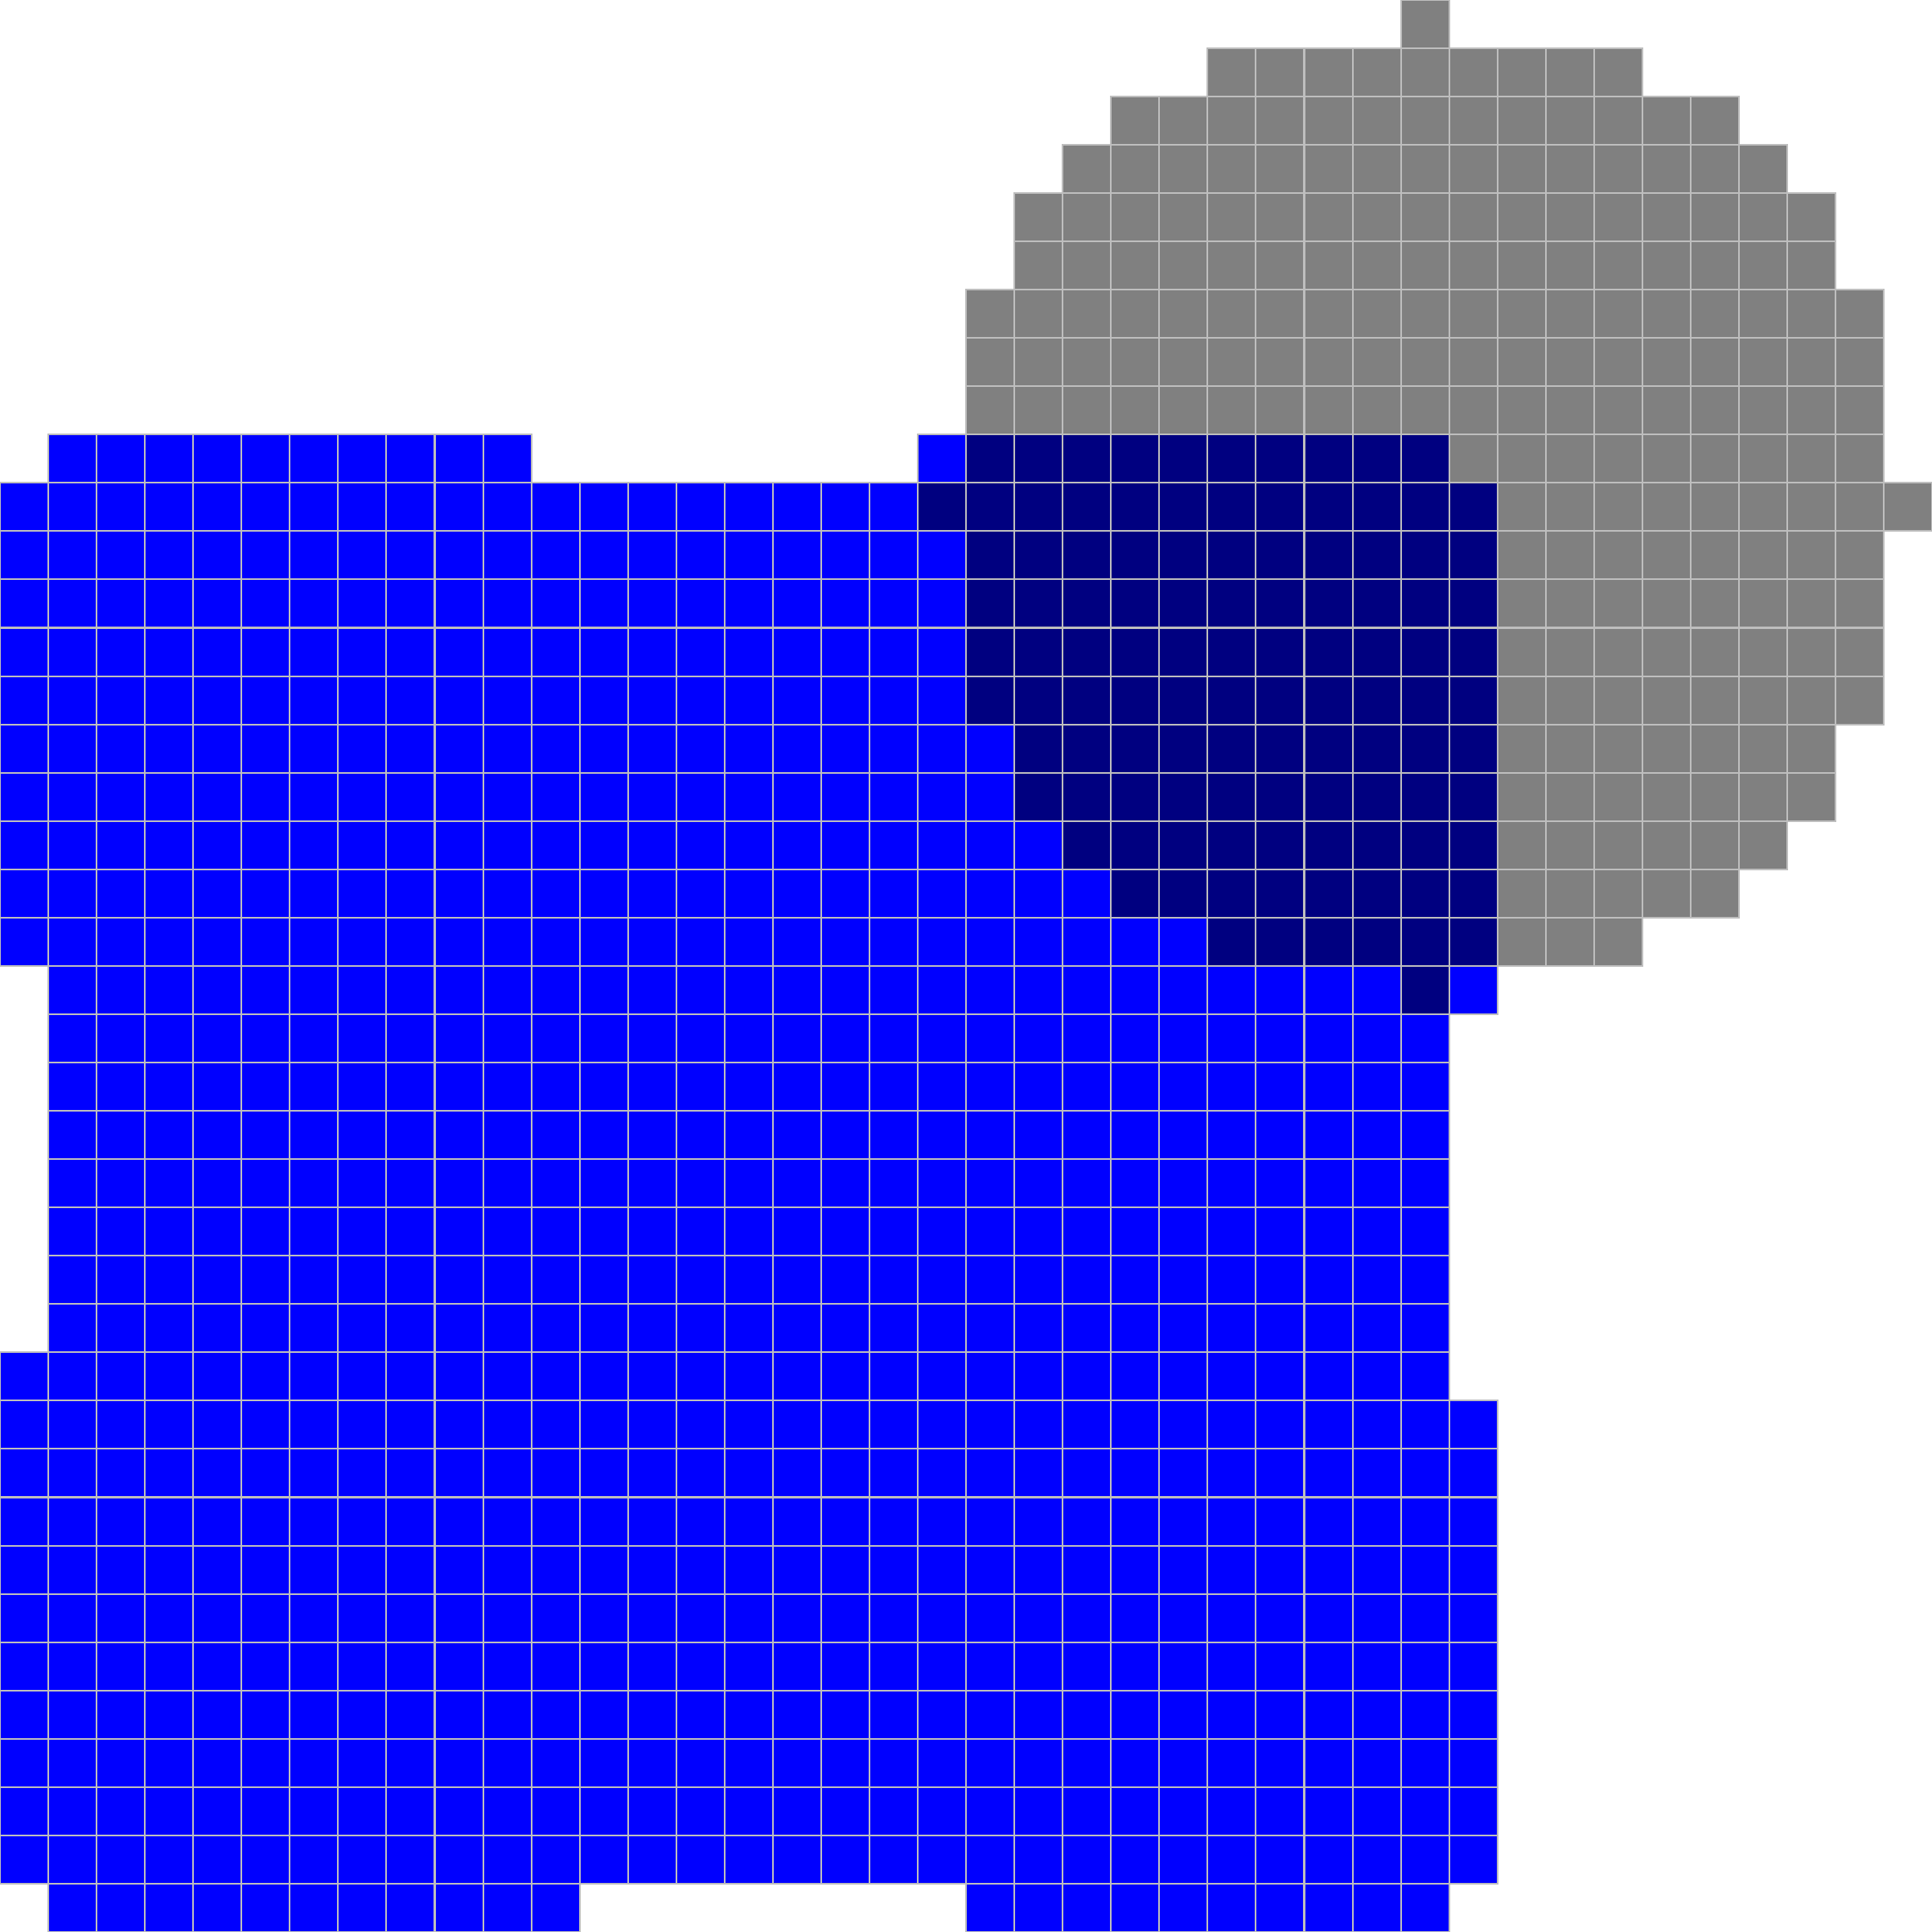
\includegraphics[scale=0.15]{figures/chapter6/contour-information/after-opt.pdf}
\label{ch6:fig:contour-info-2}
\end{minipage}%
\caption{ \daniel{\textbf{Fixed boundary evaluation.}} The proposed model does not take contour information into account, thus the II curvature estimator is evaluated and optimized with respect the initial boundary. In the left, the initial shape and the optimization variables colored in yellow. In the right, the final shape without taking the complementary solution.}
\label{ch6:fig:contour-info}
\end{figure}
\daniel{We are going to justify~\cref{ch6:alg:evolution-model} considering the case in which $m=0$, i.e., for energy $E_{\theta,0}^{flip}$. } As discussed in~\cref{ch5:sec:global-optimization}, the topological constraints are a fundamental part in a global optimization model for the digital elastica but the complexity added to it dampens any hope of optimizing it efficiently. In the proposed FlipFlow model, we exclude topological constraints and we end up with the tractable binary second order~\cref{eq:energy-family}. However, due the lack of contour information, the minimization of~\cref{eq:energy-family} for $\Ds^{(k)}$ results in undesirable shapes of even higher digital elastica energy values  (see~\cref{ch6:fig:contour-info}). Interestingly, by using the inverse of the optimal assignement, we can derive a shape of lower digital elastica energy. Therefore, the next shape is given by
\begin{align*}
	\Ds^{(k+1)} = \daniel{F^{(k)} + } \argmin _{}{E_{(\vec{\theta},m)}^{flip}\big(\Ds^{(k)},1-X^{(k)}} \big).
\end{align*}
%
Recall that the integral invariant estimator approaches curvature by computing the difference between half of the area
of a chosen ball and the area of the intersection of this ball with the shape.  In particular, regions of positive
curvature have fewer pixels in their intersection set than on its complement w.r.t the estimation ball. This implies
that variables in such regions are labeled with 1, as the unbalance grows otherwise. We attenuate curvature if we shift
the center of the estimation ball towards the interior of the shape, which means to remove the 1-labeled pixels. That is
why we take the complement of the optimization solution.


The explanation above covers the treatment of convex parts, but the way to treat concavities is not much different. Indeed, concave regions are convex in the shape complement. The FlipFlow~\cref{ch6:alg:evolution-model} is made of two modes: shrink and expansion. The shrink mode handles convexities and its reasoning is explained in the last paragraph. The expansion mode operates exactly in the same way, but at the image complement, and by doing this we are able to handle
concavities. It is called expansion mode because the optimization region, in this case, is the outer pixel boundary of
the original shape. Table~\cref{tab:flow-summary} sums up these arguments.

%Length and data terms should be properly defined in order to comply with the complement step of the FlipFlow
%algorithm. The length penalization is defined as
%
%\begin{align}
%  s(x_{w(p)})=\sum_{q \in \mathcal{N}_4(p)}{ t(q) }, \quad \text{where } t(q) = \left\{\begin{array}{ll}
%  (x_{w(p)}-x_{w(q)})^2, & \text{if } q \in I^{(k)}\\
%  (x_{w(p)}-0), & \text{if } q \in F^{(k)}\\
%  (x_{w(p)}-1), & \text{otherwise }
%  \end{array}\right.
%  \label{eq:length-penalization}
%\end{align}
%
\begin{table}
  \center
  \setlength{\extrarowheight}{0.75em}
  \begin{tabular}{|c|c|c|c|} \hline
    shrink mode &    $\kappa \gg 0$ & $\kappa \geq 0$ &  $\kappa < 0$ \\ \hline
    $x^{(k)}$ & $x_j=1$ & $x_j \in \{0,1\}$ & $x_j=0$ \\ \hline
    $\Ds^{(k+1)} \leftarrow F^{(k)} + x^{(k)}$ & eroded & prob. eroded & unchanged  \\ \hline \hline
    expansion mode &    $\overline{\kappa} \gg 0$ & $\overline{\kappa} \geq 0$ & $\overline{\kappa} < 0$ \\ \hline
    $\overline{x}^{(k)}$ & $\overline{x}_j=1$ & $\overline{x}_j \in \{0,1\}$ & $\overline{x}_j=0$ \\ \hline
    $\Ds^{(k+1)} \leftarrow \overline{\overline{F}^{(k)} + \overline{x}^{(k)}}$ & dilated & prob. dilated & unchanged \\ \hline 
  \end{tabular}
  
  \caption{ \daniel{\textbf{Shrink and expansion modes.}} Since the curvature is negated when reversing the curve (i.e. $\overline{\kappa}=-\kappa$), this process can only shrink  convex parts in shrink mode and expand concave parts in expansion mode.}
   \label{tab:flow-summary}	  

\end{table}


In~\cref{ch6:fig:m1-square-flow} we show the results of the FlipFlow algorithm for $( \daniel{m=0}, \alpha=\{0, 0.5\}, \beta=1 )$. We observe a global evolution towards rounder shapes, but several artifacts are formed along the boundary. An estimation ball of higher radius evolves the shapes faster, but the contours become noisier. Setting $\alpha >0$ attenuates the problem for lower radius but the produced shapes does not match with our intuition of what a flow driven by the squared curvature must be like. In the next section we investigate how the energy properties and optimization method used can explain this behavior.

\begin{figure}
\center
\begin{tabular}{p{2.5em}ccc}
& $r=3$ & $r=5$ & $r=9$ \\[2em]
\multirow{2}{*}{$\alpha=0$}& 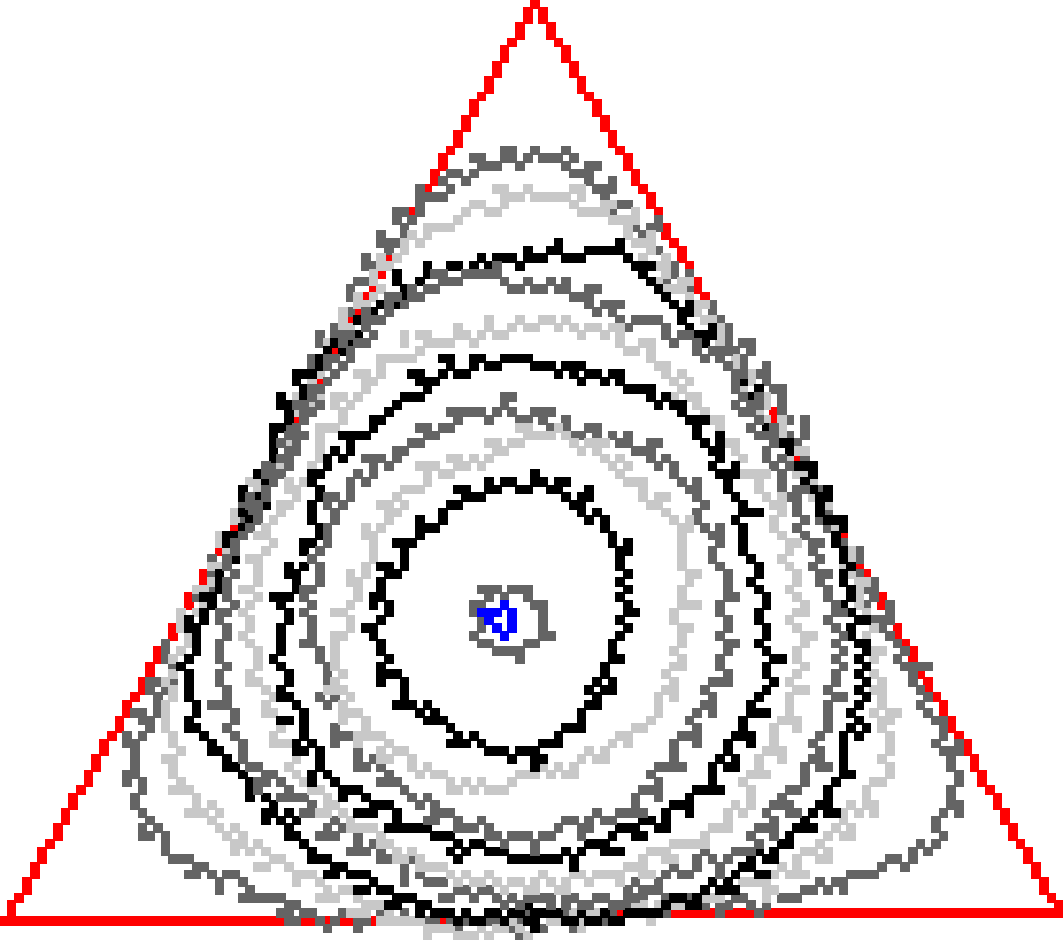
\includegraphics[scale=0.25]{figures/chapter6/radius-effect/triangle/improve/len_pen0/radius-3/summary.pdf} &
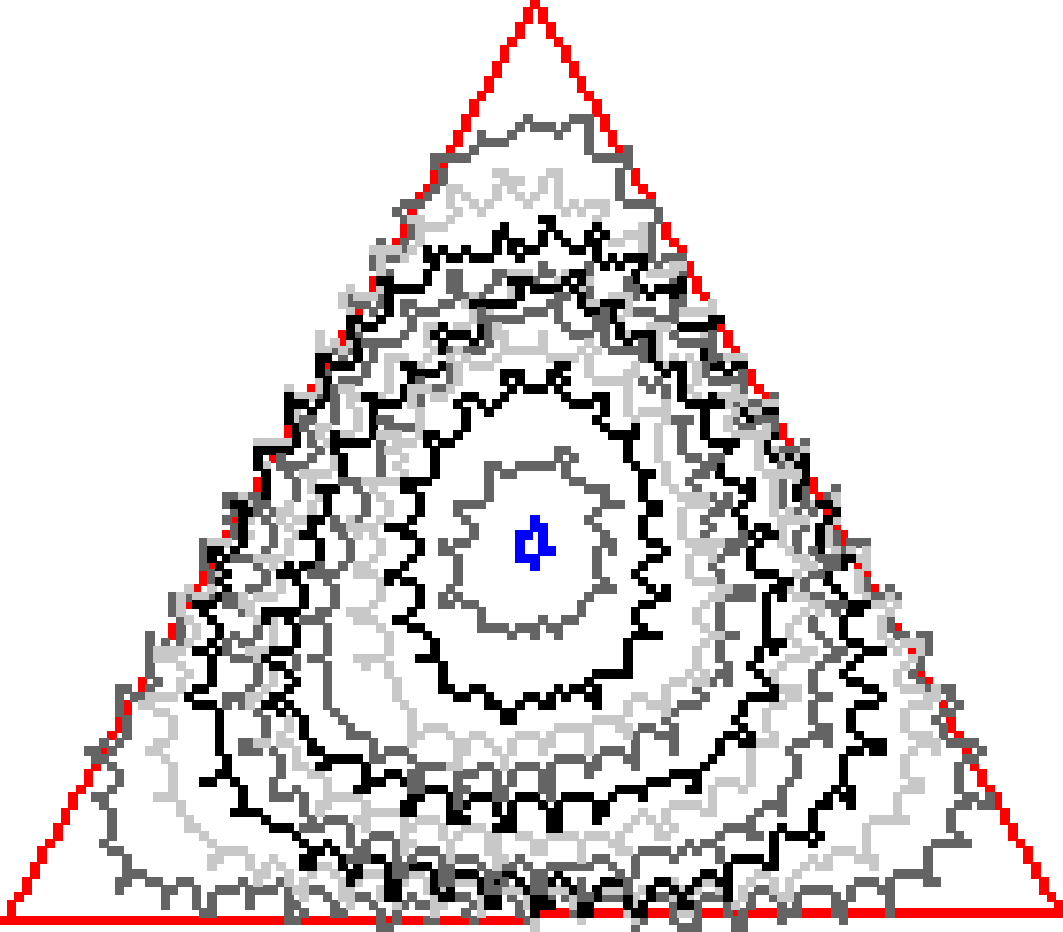
\includegraphics[scale=0.23]{figures/chapter6/radius-effect/triangle/improve/len_pen0/radius-5/summary.pdf} &
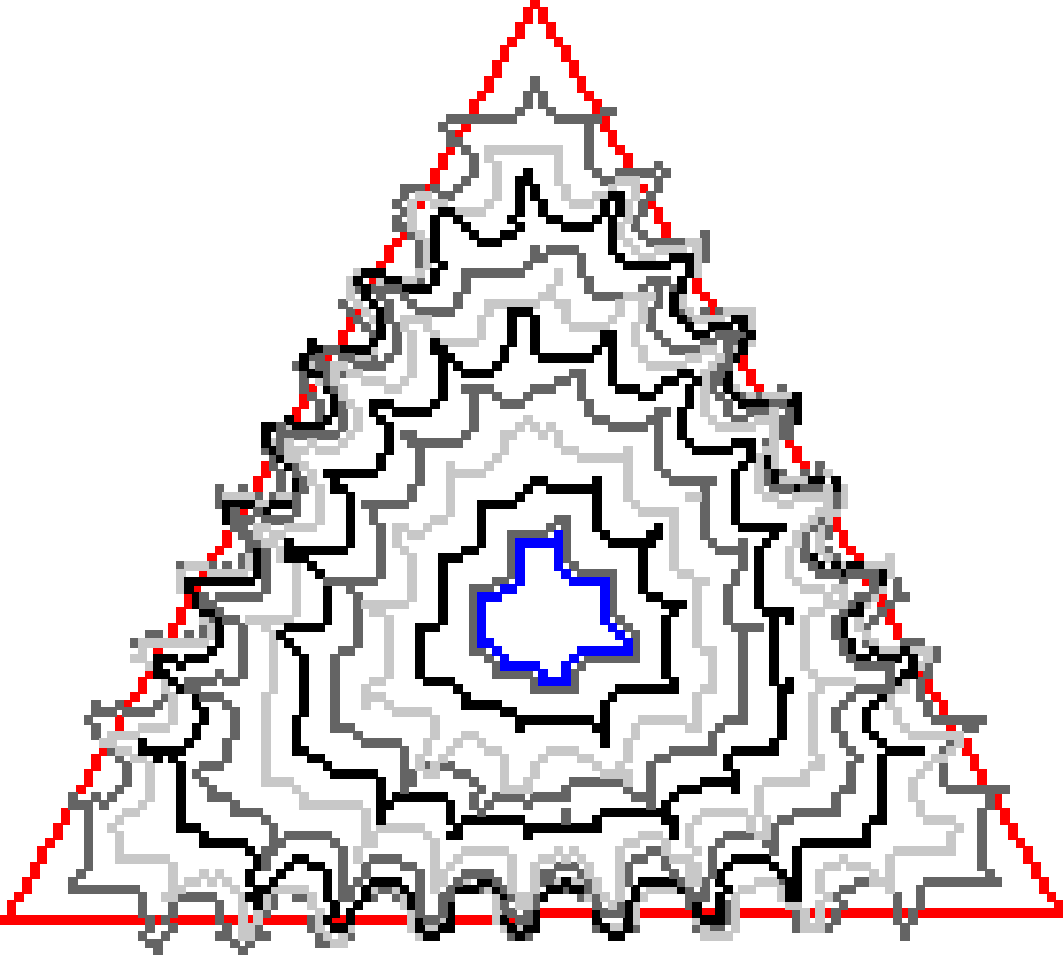
\includegraphics[scale=0.23]{figures/chapter6/radius-effect/triangle/improve/len_pen0/radius-9/summary.pdf} \\[2em]
& 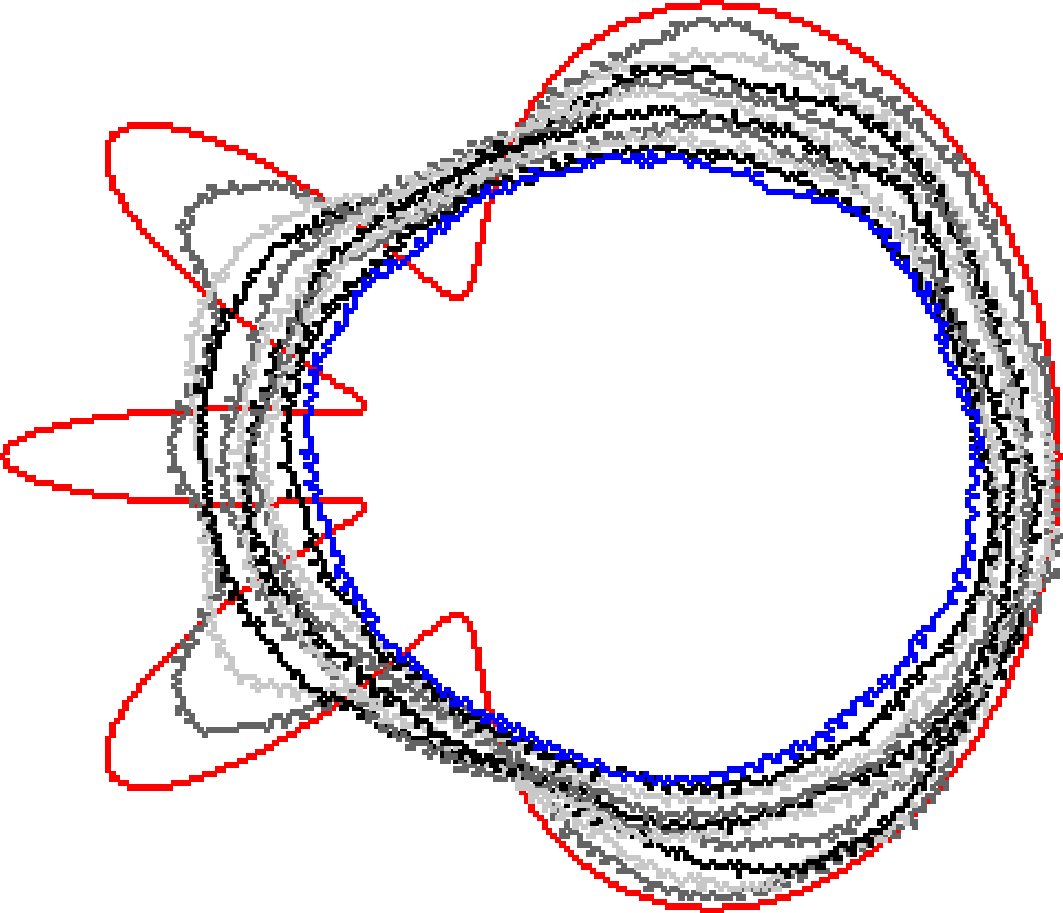
\includegraphics[scale=0.23]{figures/chapter6/radius-effect/flower/improve/len_pen0/radius-3/summary.pdf} &
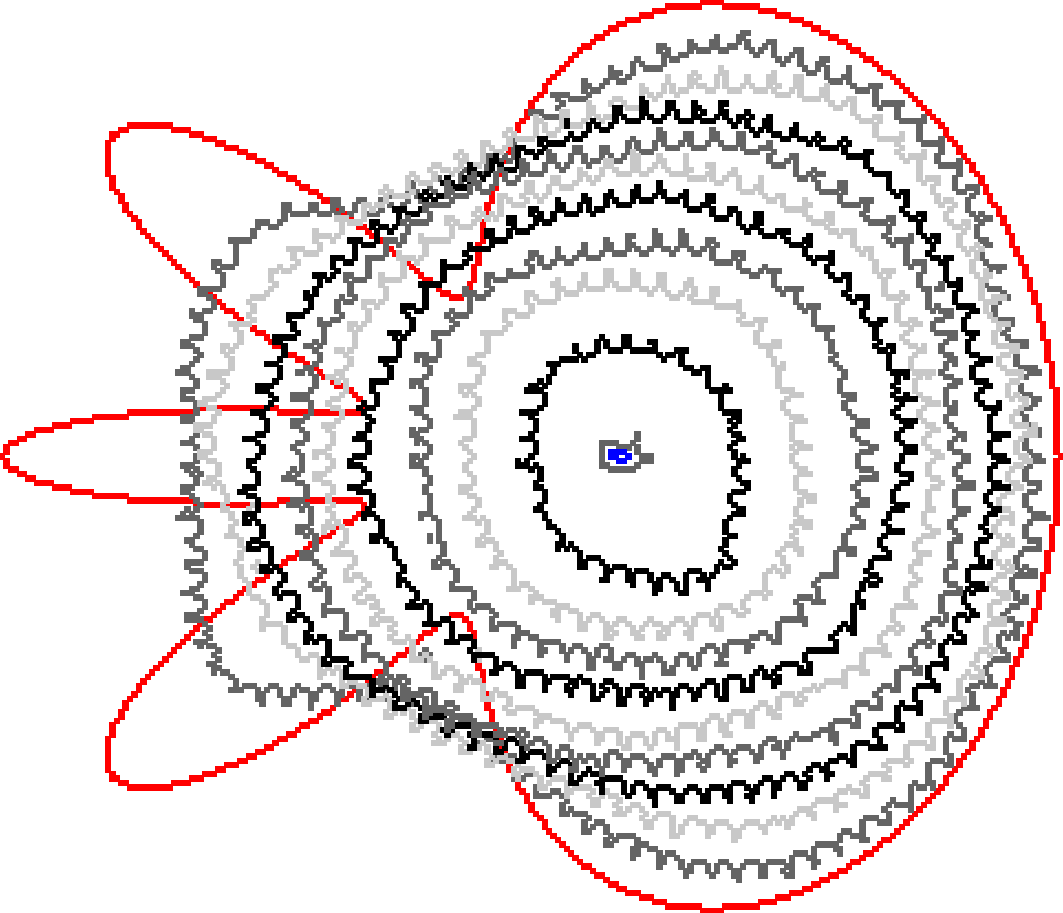
\includegraphics[scale=0.23]{figures/chapter6/radius-effect/flower/improve/len_pen0/radius-5/summary.pdf} &
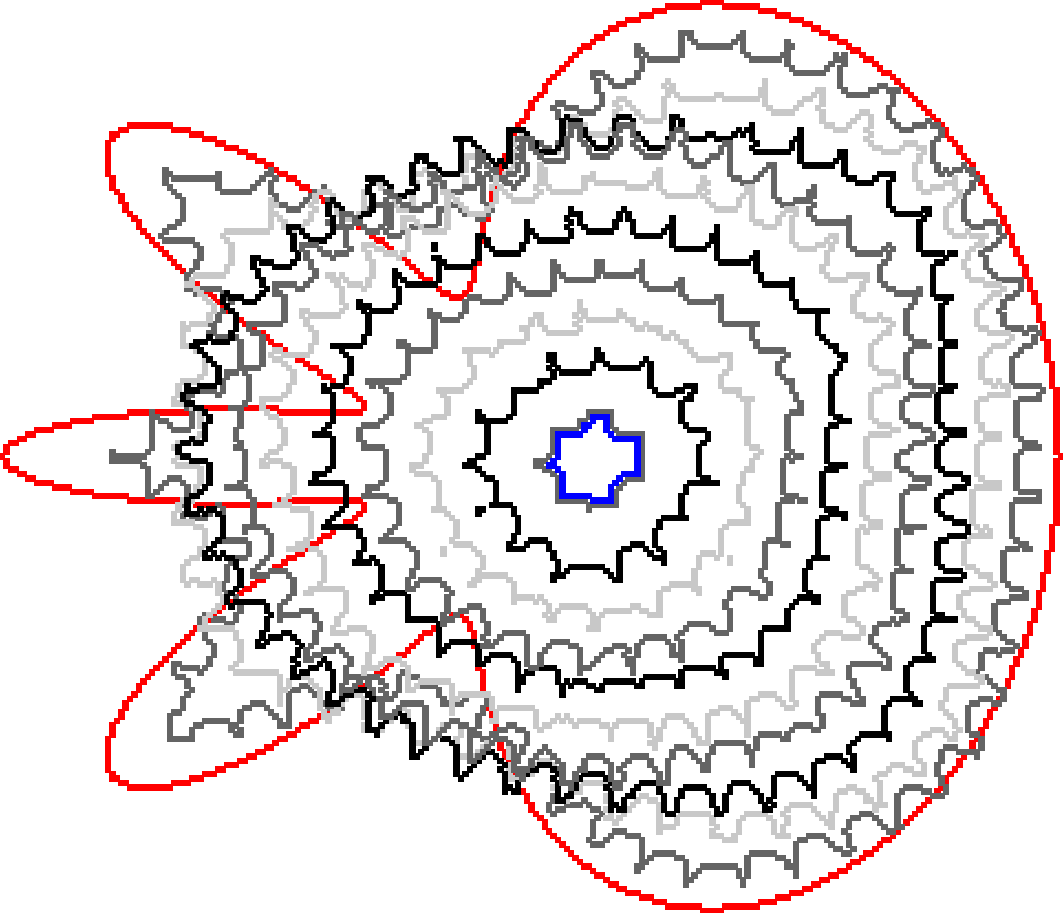
\includegraphics[scale=0.23]{figures/chapter6/radius-effect/flower/improve/len_pen0/radius-9/summary.pdf} \\
\hline \\
\multirow{2}{*}{$\alpha=0.5$}& 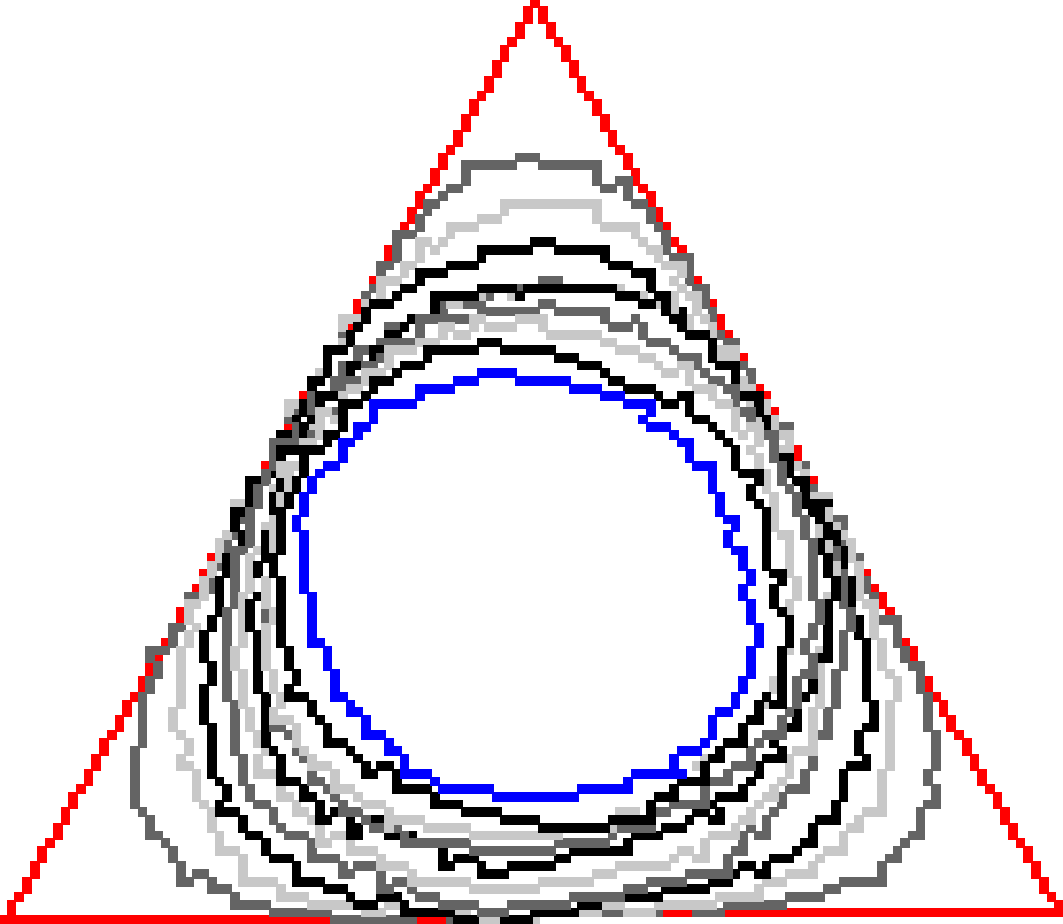
\includegraphics[scale=0.25]{figures/chapter6/radius-effect/triangle/improve/len_pen0.5/radius-3/summary.pdf} &
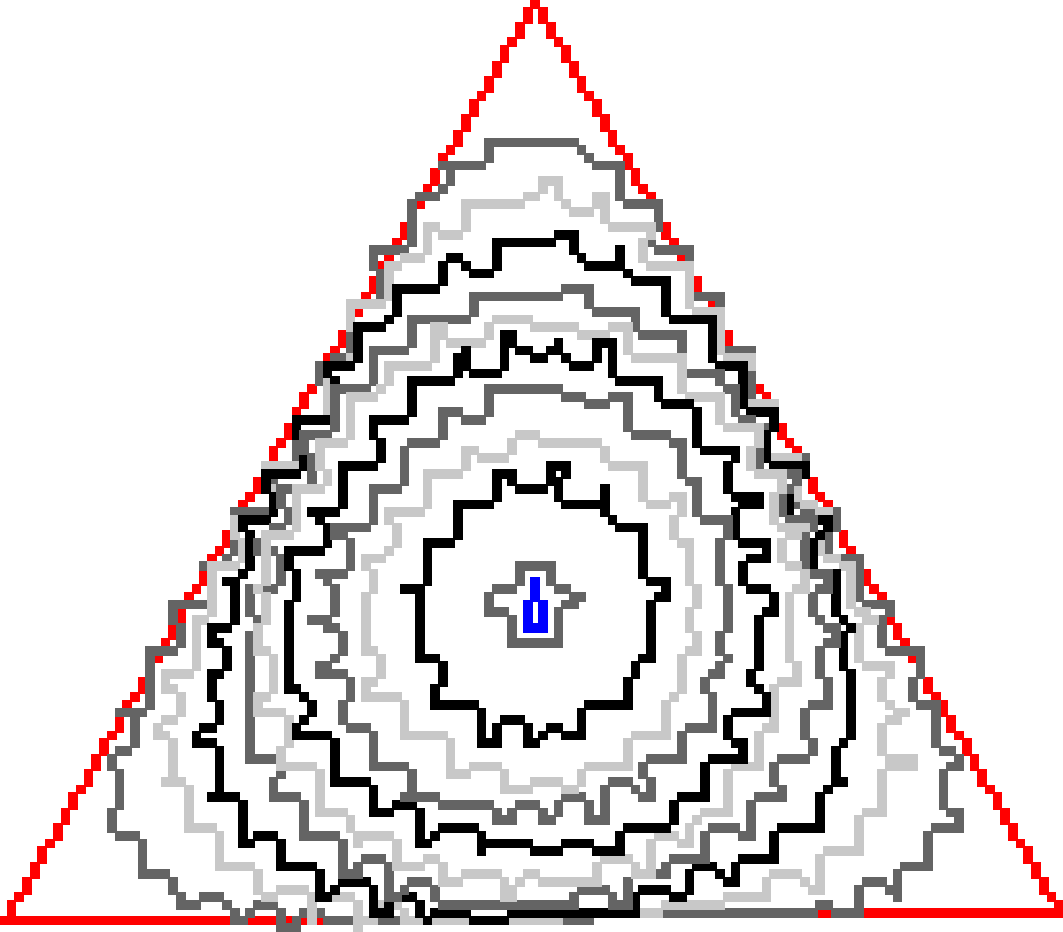
\includegraphics[scale=0.23]{figures/chapter6/radius-effect/triangle/improve/len_pen0.5/radius-5/summary.pdf} &
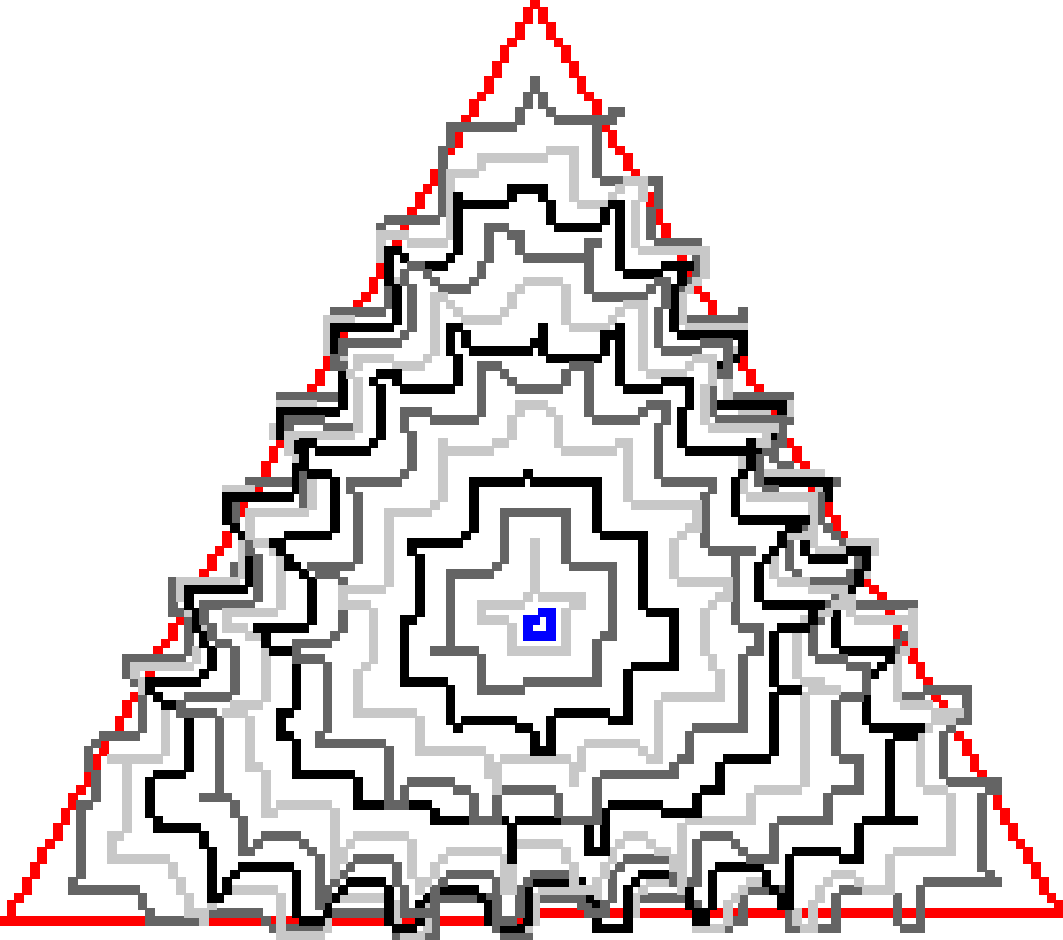
\includegraphics[scale=0.23]{figures/chapter6/radius-effect/triangle/improve/len_pen0.5/radius-9/summary.pdf} \\[2em]
& 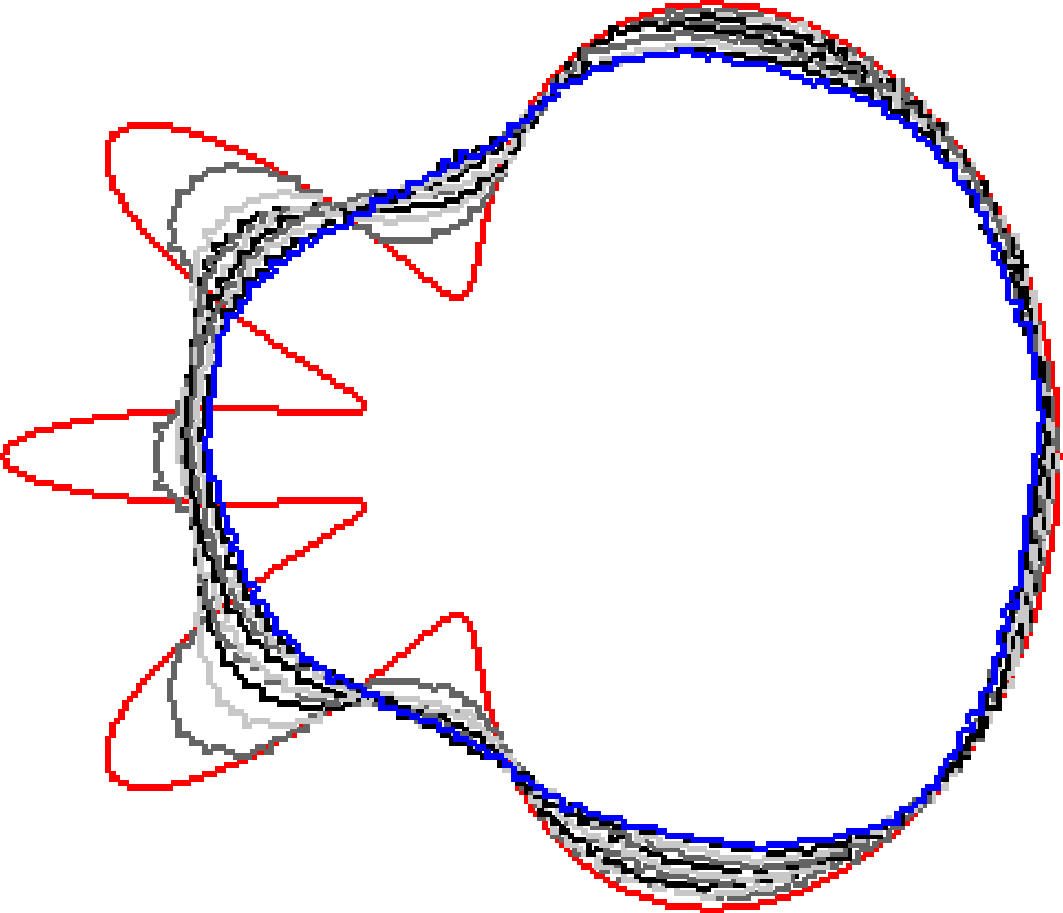
\includegraphics[scale=0.23]{figures/chapter6/radius-effect/flower/improve/len_pen0.5/radius-3/summary.pdf} &
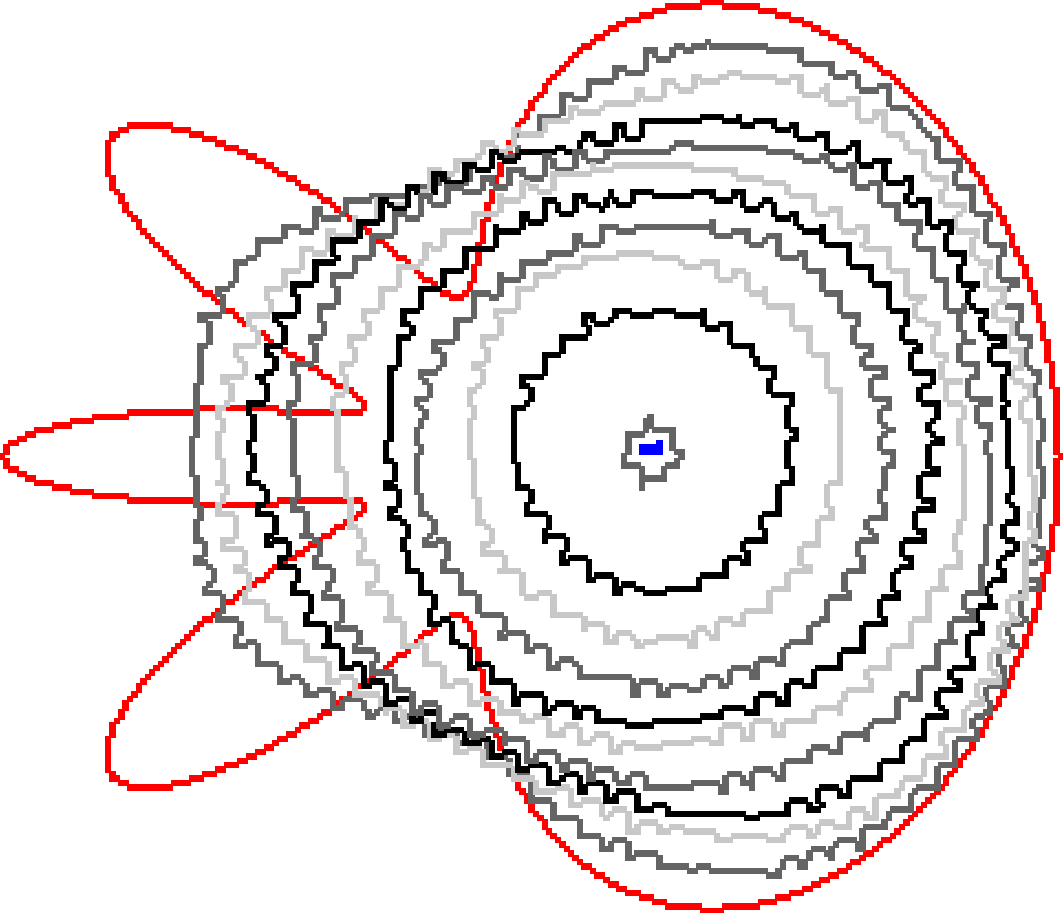
\includegraphics[scale=0.23]{figures/chapter6/radius-effect/flower/improve/len_pen0.5/radius-5/summary.pdf} &
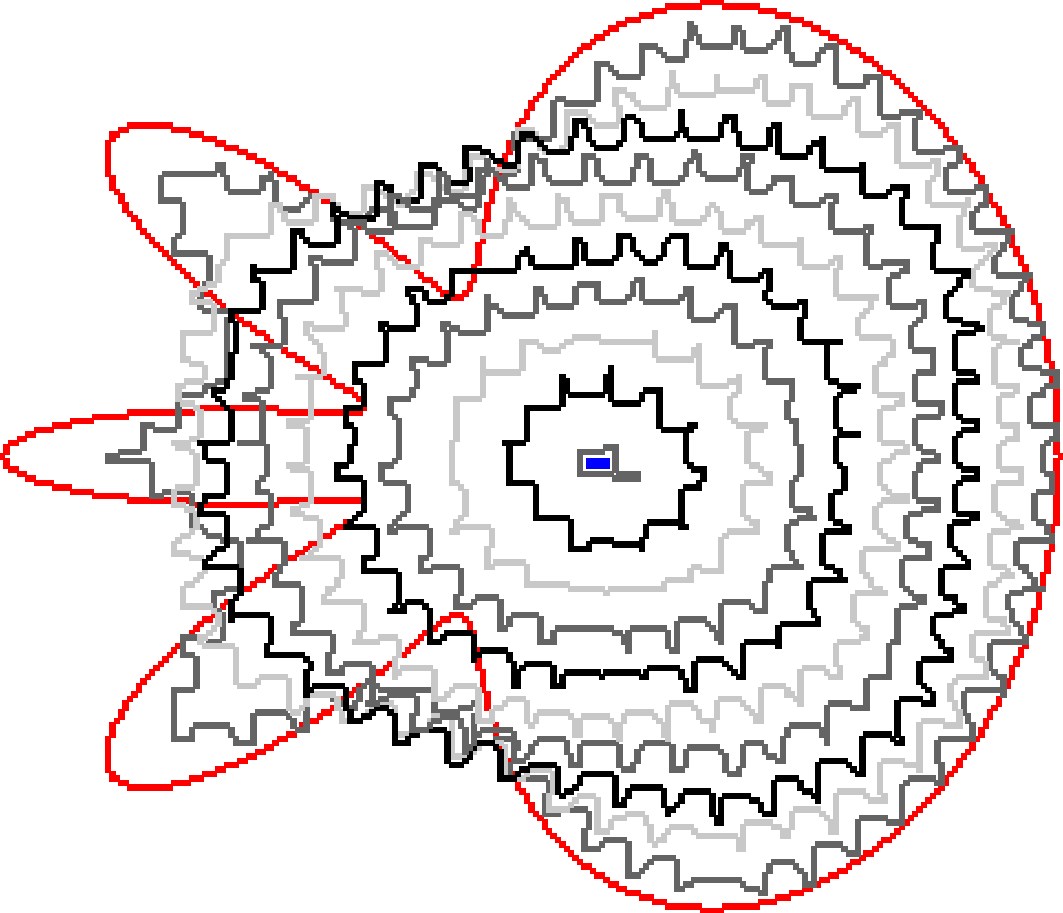
\includegraphics[scale=0.23]{figures/chapter6/radius-effect/flower/improve/len_pen0.5/radius-9/summary.pdf}
\end{tabular}

\caption{\daniel{\textbf{FlipFlow results for $m=0,\beta=1$.}} The algorithm is very sensitive to the little variations of the estimator, which are particularly important in regions of low squared curvature. Artifacts are somewhat reduced with a length penalization but increases if we use a higher ball radius. For better visualization, curves are displayed every $1/10$ of the number of iterations. }
\label{ch6:fig:m1-square-flow}
\end{figure}


%\begin{figure}
%\center
%\subfloat[]{
%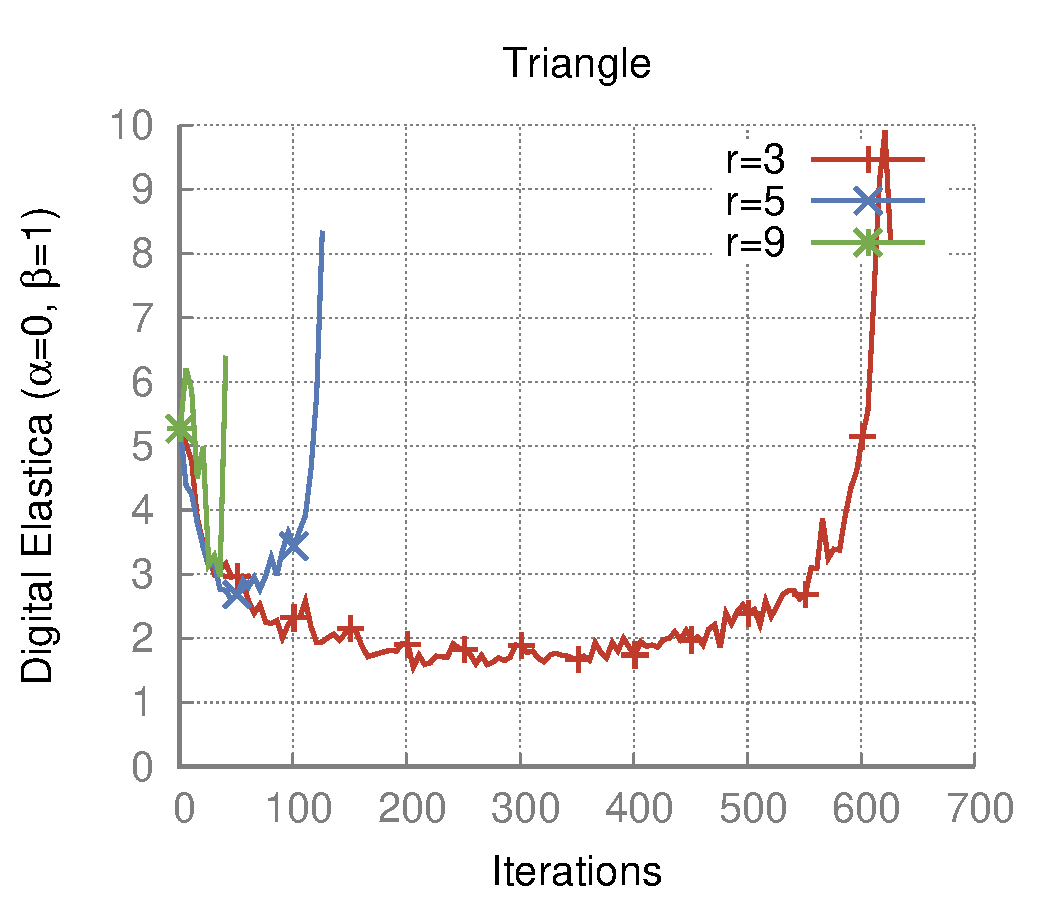
\includegraphics[scale=0.45]{figures/chapter6/radius-effect/triangle/improve/len_pen0/radius-3/radius-effect.pdf}}%
%\subfloat[]{
%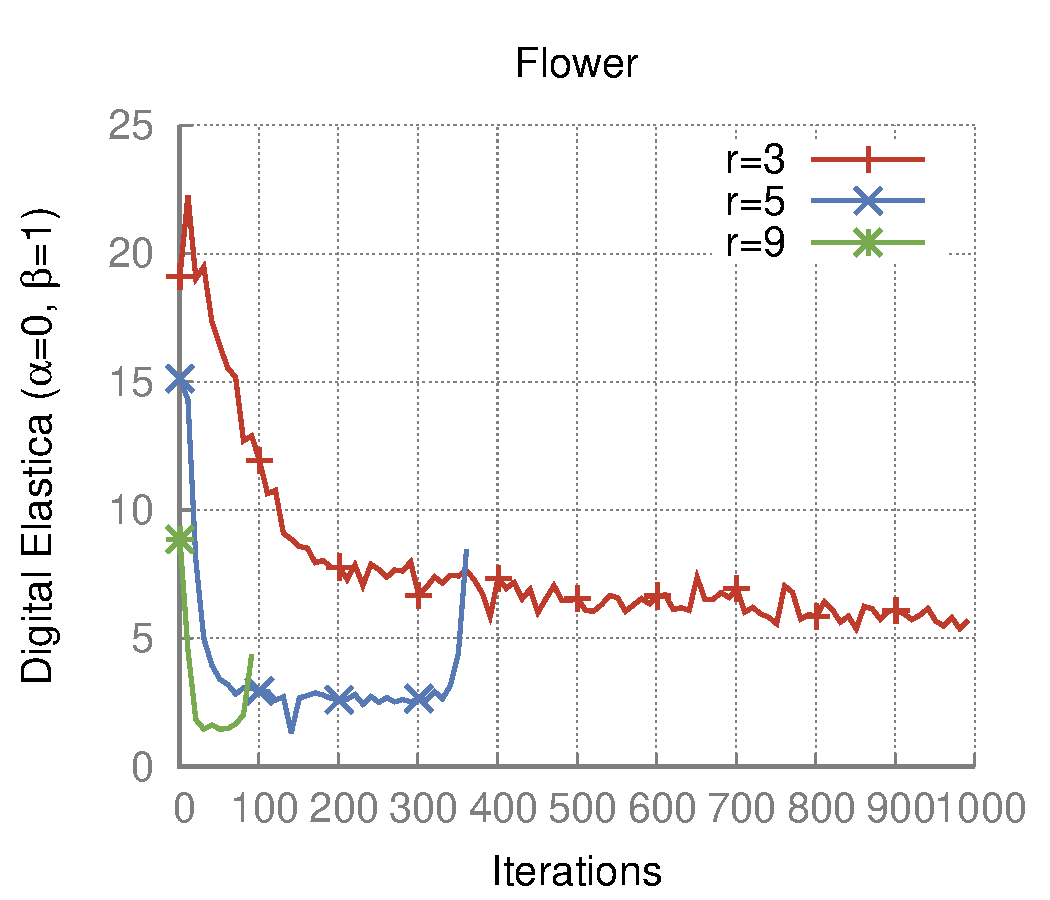
\includegraphics[scale=0.45]{figures/chapter6/radius-effect/flower/improve/len_pen0/radius-3/radius-effect.pdf}}%
%\caption{The digital elastica decreases in a turbulent way.}
%\end{figure}


\section{Optimization method}
\label{ch6:sec:optimization-method}

Let $f$ be a function of $n$ binary variables with unary and pairwise terms, i.e.
\begin{align*}
f(y_1,\cdots, y_n) = \sum_{j}{f_j(y_j)} + \sum_{j < k}{f_{j,k}(y_j,y_k)}.
\end{align*}
%
\daniel{As observed in~\cref{ch2:sec:pseudo-boolean-functions},} function $f$ is submodular if and only if the following inequality holds for each pairwise term $f_{j,k}$: %\cite{kolmogorov04whatenergies}
\begin{align*}
  \quad f_{j,k}(0,0) + f_{j,k}(1,1) \leq f_{j,k}(0,1) + f_{j,k}(1,0).
\end{align*}
%
The energy $E_{(\vec{\theta},m)}^{flip}$ is non-submodular and optimizing it is a difficult problem, which constrains us to use heuristics and
approximation algorithms. The QPBO method \cite{hammer84} transforms the original problem in a max-flow/min-cut
formulation and yields a full optimal labeling for submodular energies. For non-submodular energies the method is
guaranteed to return a partial labeling with the property that the set of labeled variables is part of an optimal
solution. That property is called partial optimality.

In practice, QPBO can leave many pixels unlabeled. There exist two extensions to QPBO that alleviate this limitation:
QPBOI (improve) and QPBOP (probe) \cite{rother07qpbo}. The first is an approximation method that is guaranteed to not increase the energy,
but loses the property of partial optimality. The second is an exact method which is reported to label more variables
than QPBO.

The percentage of unlabeled pixels by QPBOP for $E_{(\vec{\theta},m)}^{flip}$ is quite high, but the percentage decreases to zero as we set $m$
to a value closer to $r$, the estimation ball radius. Therefore, we are more confident in taking the solution for values of $m$ close to $r$. However, the way it
varies across values of $m$ differs from shape to shape, as is illustrated in~\cref{ch6:fig:unlabeled-versus-iterations}. We also noticed that, for $m=r$, all the pixels were labeled, which
  indicates that $E_{(\vec{\theta},r)}^{flip}$ is an easy instance of the general non-submodular energy $E_{(\vec{\theta},m)}^{flip}$, but this remains to be
  proved. The number of pairwise terms in $E_{(\vec{\theta},r)}^{flip}$ is roughly half of those in $E_{(\vec{\theta},1)}^{flip}$ (see~\cref{ch6:fig:ratio-pairwise-terms}), which also explains the higher number of labeled variables.

  We have used QPBOI to solve $E_{(\vec{\theta},m)}^{flip}$. Naturally, in the case where all pixels are labeled by QPBOP, QPBOI returns the same labeling as QPBOP. In the next section we show that by evaluating the estimation ball at outer rings, we eliminate the artifacts and we produce smoother flows while preserving a qualitative measure of curvature.
  
  \daniel{We postpone the comparison of the proposed methods in this thesis to~\cref{chapter:results-analysis}. At this point, we retain us to say that the FlipFlow performs up to 10x faster than the LocalSearch algorithm.} 


\begin{figure}
\center
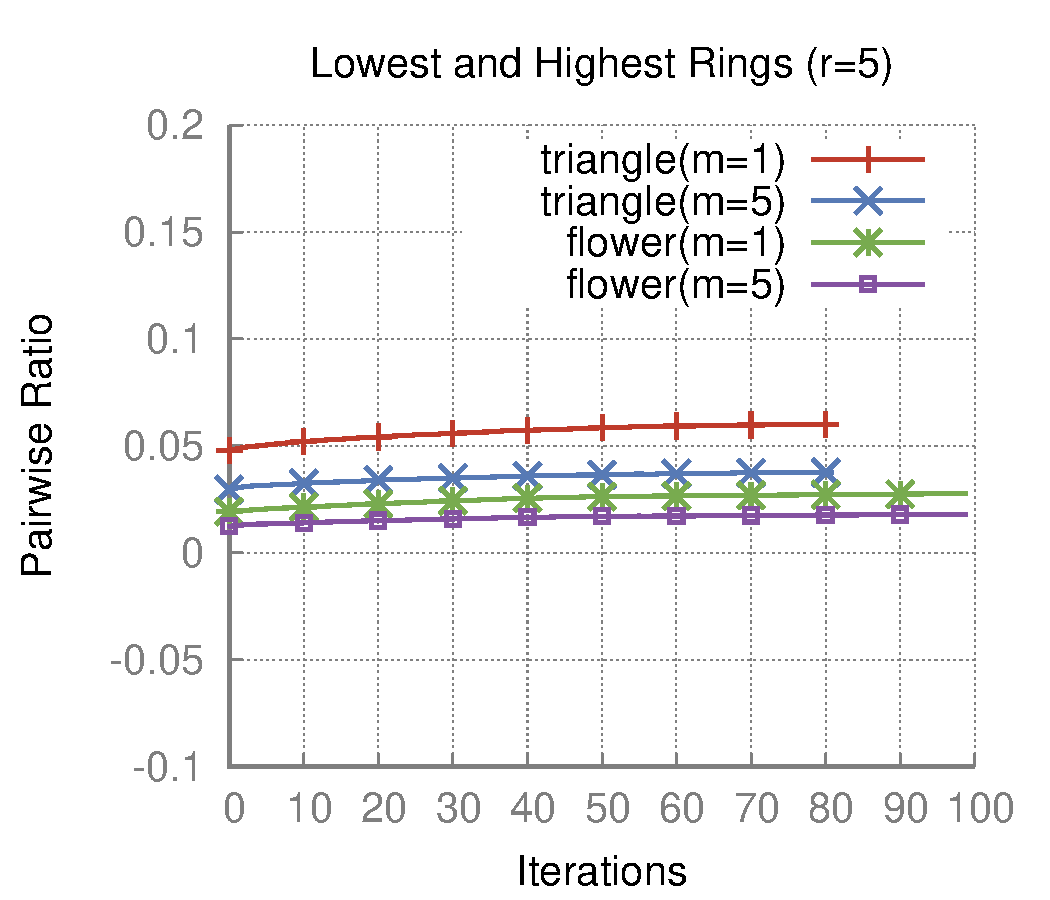
\includegraphics[scale=0.5]{figures/chapter6/unlabeled-ratio/plots/pairwise-ratio/h0.25/radius-5/plot-pairwiseratio-lowerHigher-concavities-probe.pdf}
\caption{\daniel{\textbf{Pairwise terms ratio}.}We plot the ratio of pairwise terms among all $\binom{|X^{(k)}|}{2}$ combinations. The highest ring has roughly half the number of pairwise terms as the lowest ring.}
\label{ch6:fig:ratio-pairwise-terms}
\end{figure}


\begin{figure}
\center
\begin{minipage}[b]{0.5\textwidth}
%\subfloat[]{ 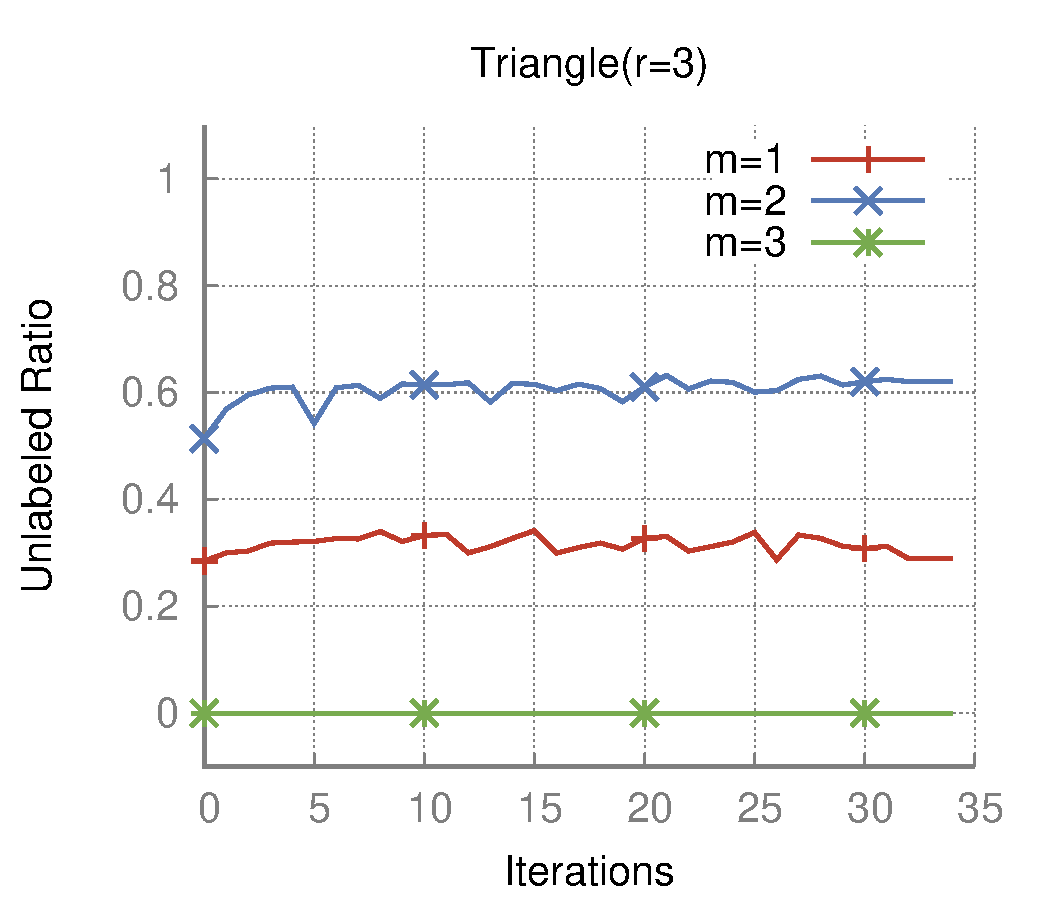
\includegraphics[scale=0.38]{figures/chapter6/unlabeled-ratio/plots/unlabeled-per-iterations/h0.25/radius-3/plot-model-triangle-concavities-probe.pdf}}\\%
\subfloat[]{ 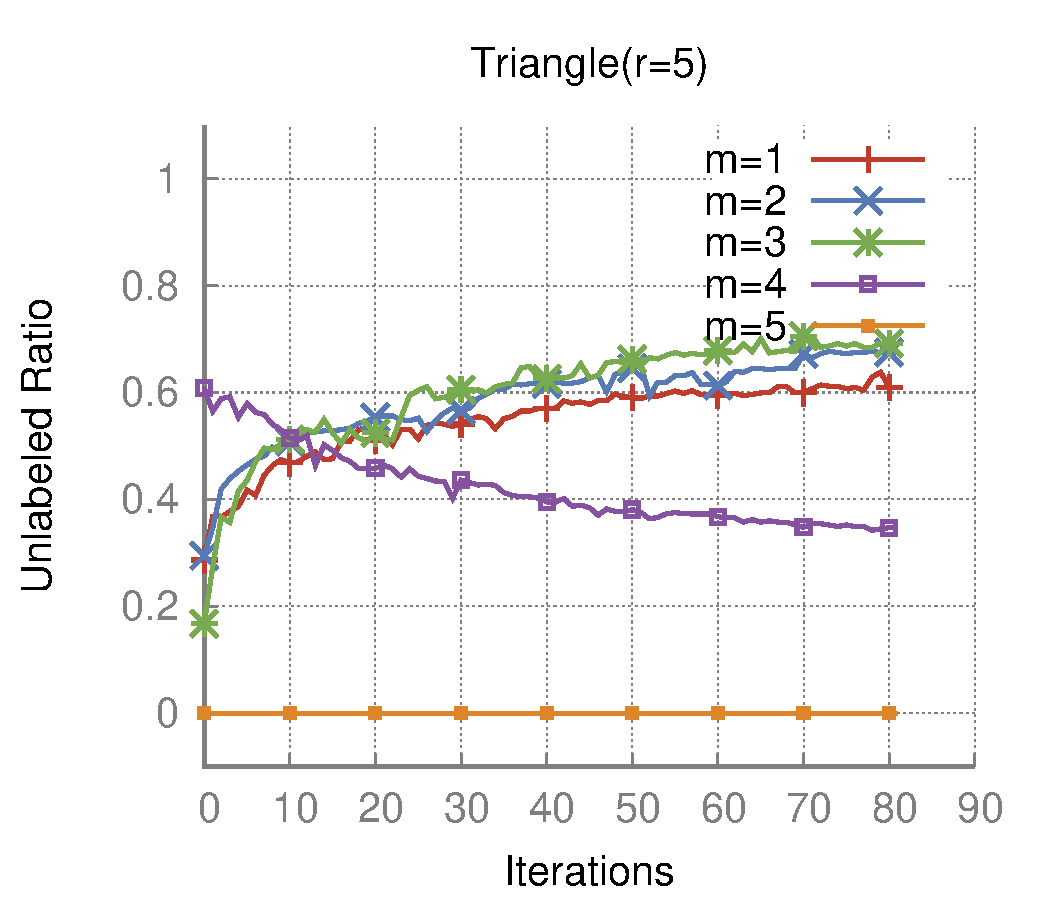
\includegraphics[scale=0.38]{figures/chapter6/unlabeled-ratio/plots/unlabeled-per-iterations/h0.25/radius-5/plot-model-triangle-concavities-probe.pdf}}\\%
\subfloat[]{ 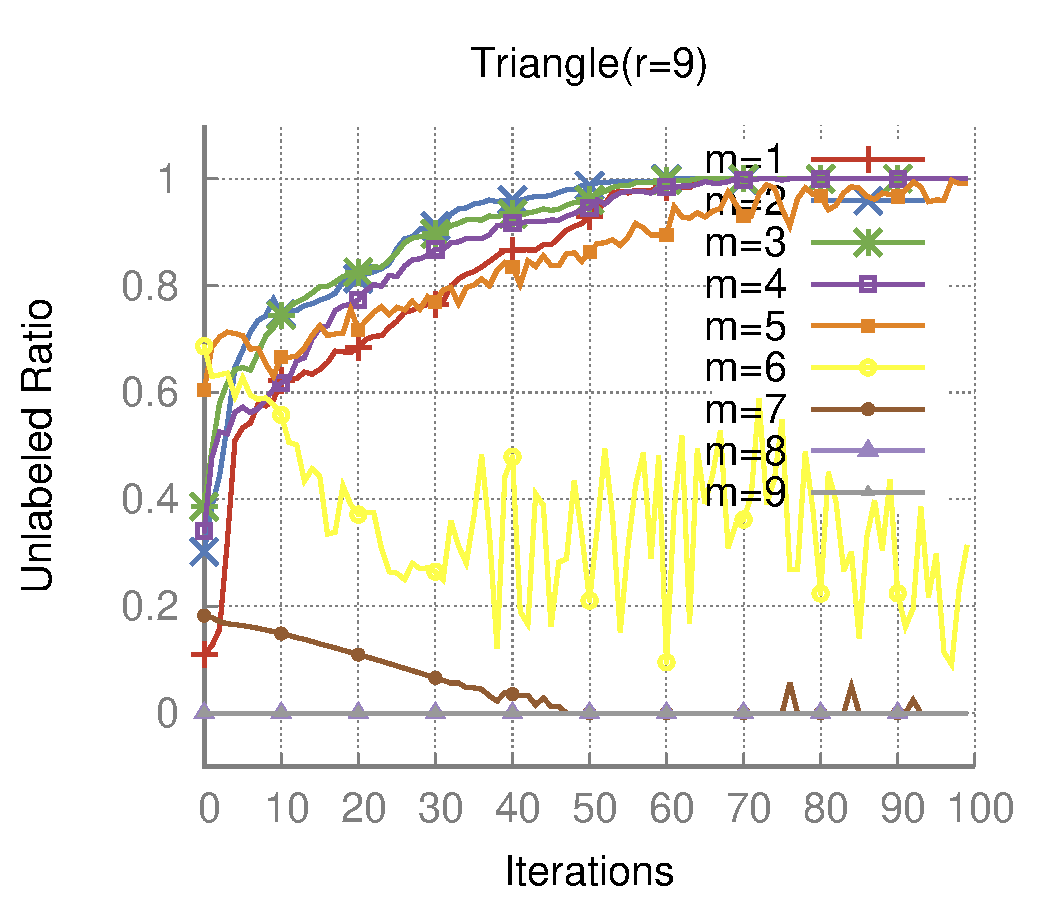
\includegraphics[scale=0.38]{figures/chapter6/unlabeled-ratio/plots/unlabeled-per-iterations/h0.25/radius-9/plot-model-triangle-concavities-probe.pdf}}%
\end{minipage}%
\begin{minipage}[b]{0.5\textwidth}
%\subfloat[]{ 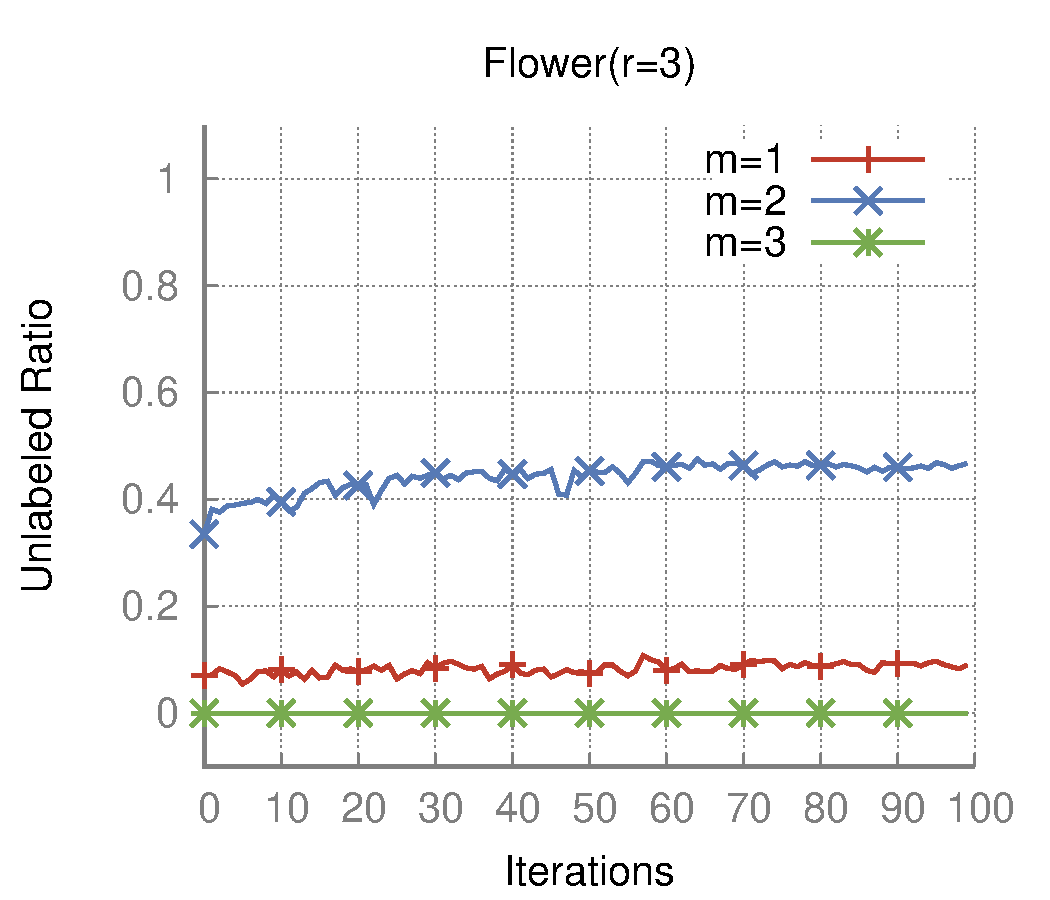
\includegraphics[scale=0.38]{figures/chapter6/unlabeled-ratio/plots/unlabeled-per-iterations/h0.25/radius-3/plot-model-flower-concavities-probe.pdf}}\\%
\subfloat[]{ 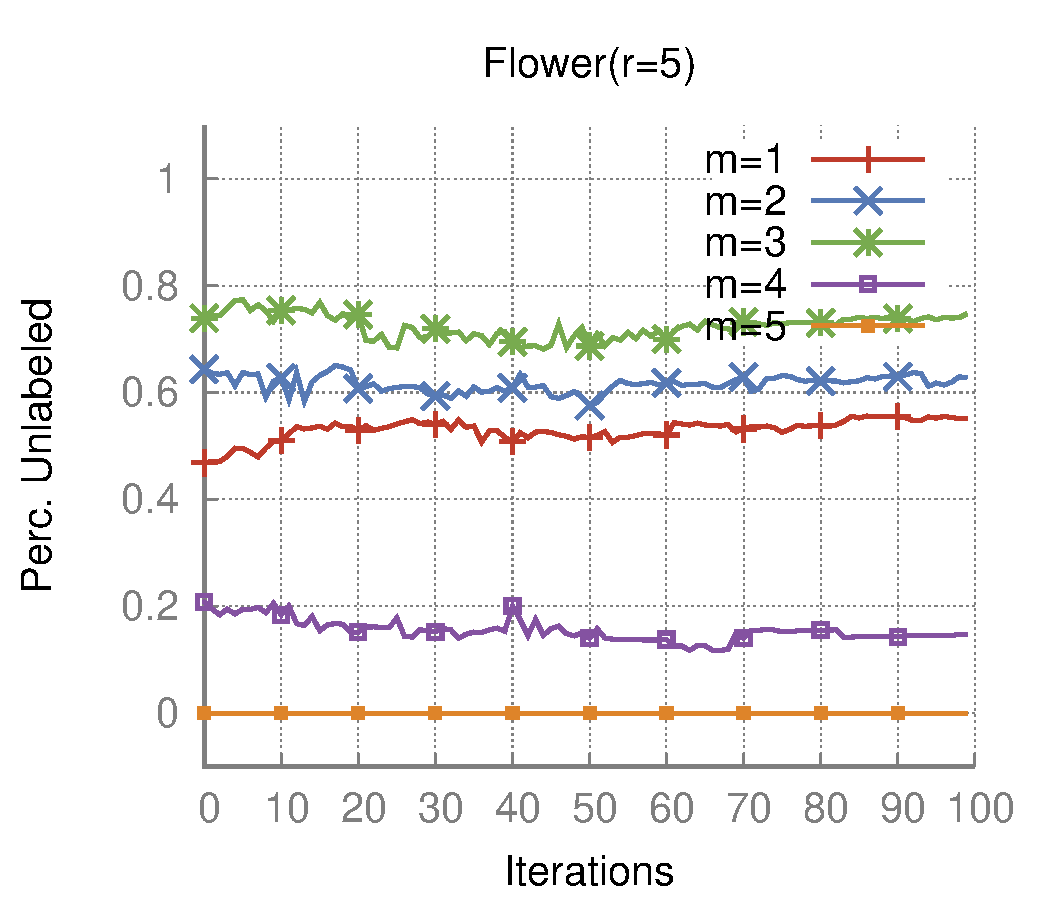
\includegraphics[scale=0.38]{figures/chapter6/unlabeled-ratio/plots/unlabeled-per-iterations/h0.25/radius-5/plot-model-flower-concavities-probe.pdf}}\\%
\subfloat[]{ 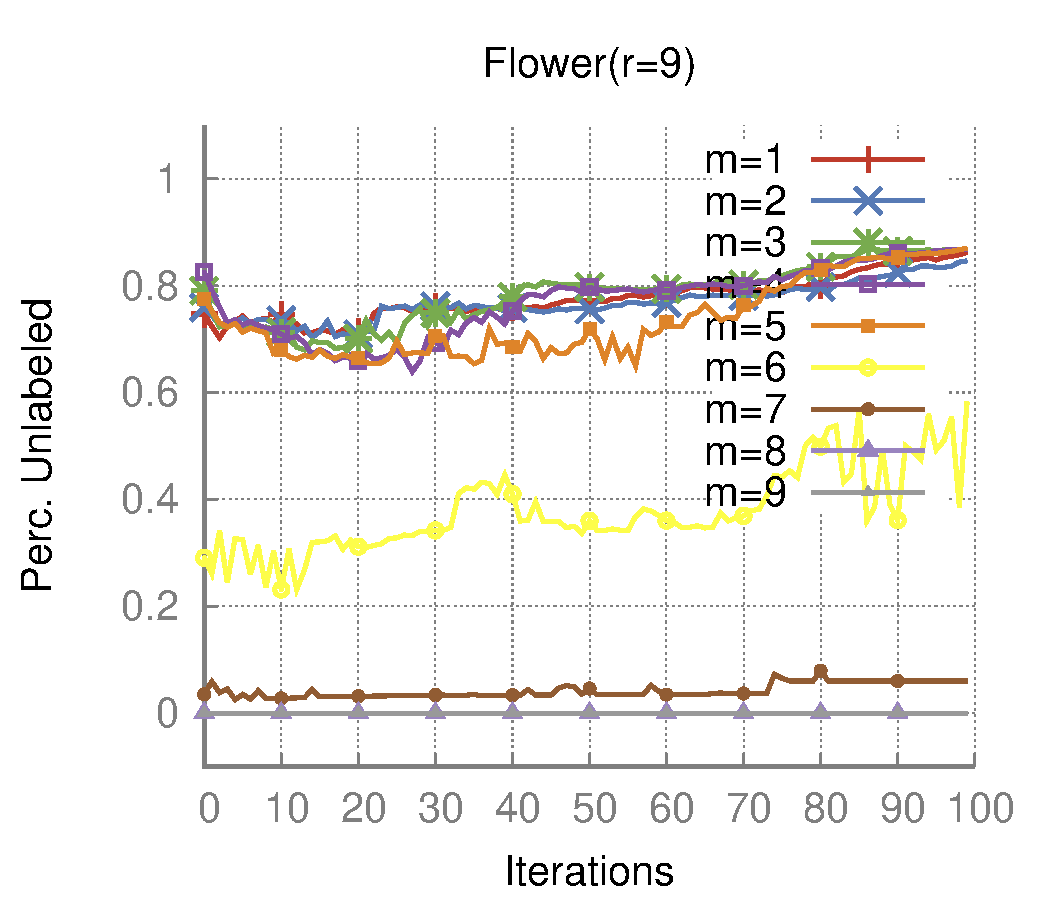
\includegraphics[scale=0.38]{figures/chapter6/unlabeled-ratio/plots/unlabeled-per-iterations/h0.25/radius-9/plot-model-flower-concavities-probe.pdf}}%
\end{minipage}
\caption{\daniel{\textbf{Unlabeled variables ratio across $m$-rings.}}For each plot, we first produce the sequence of shapes $\left\{ \Ds^{(k)} \right\}$ executing FlipFlow with $m=r$. Then, for each shape in $\left\{ \Ds^{(k)} \right\}$, we execute one iteration of FlipFlow for different values of $m$ and we count the unlabeled pixels. The number of unlabeled pixels by QPBOP remains high for lower values of $m$, and goes to zero when $m=r$. %We observe the same behavior for varying radius values.
}
\label{ch6:fig:unlabeled-versus-iterations}
\end{figure}



\section{Evaluation across $m$-rings}
\label{ch6:sec:evaluation-across-rings}

%\begin{figure}
%\center
%\begin{tabular}{p{3em}ccc}
%$m=1$ & 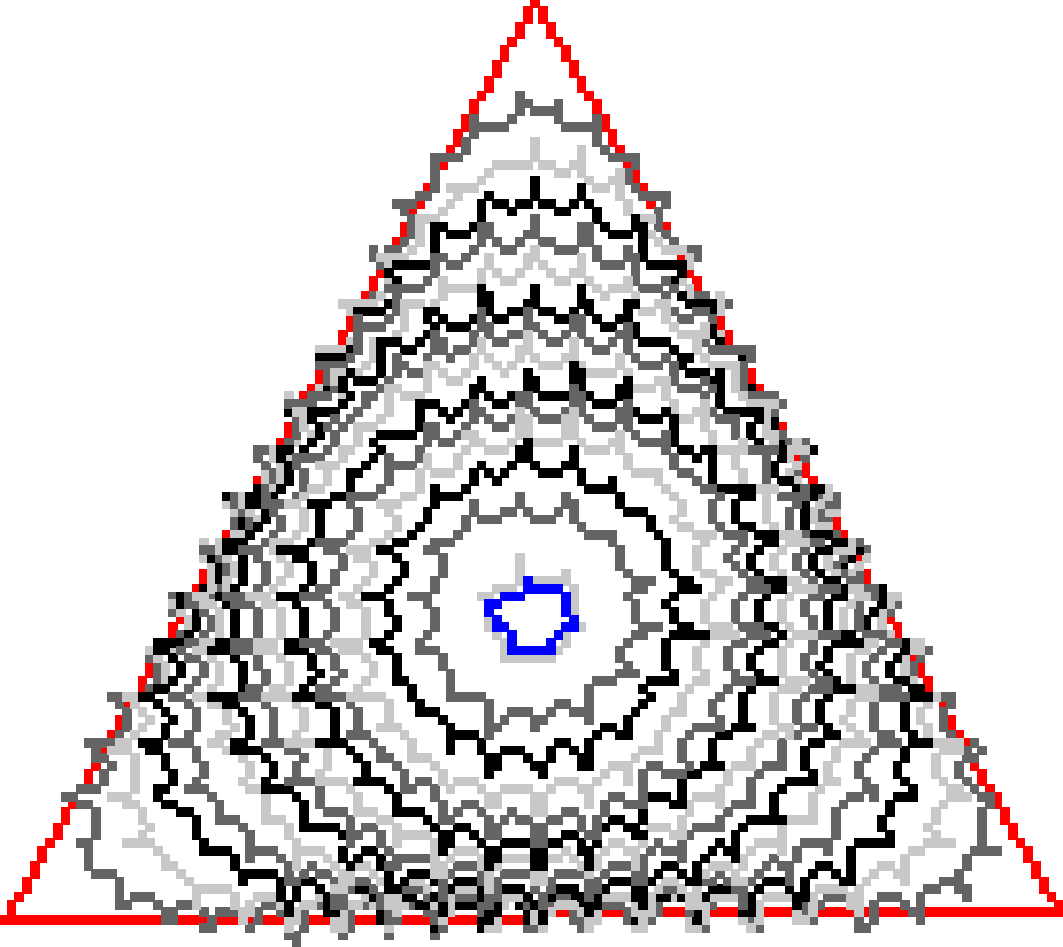
\includegraphics[scale=0.22]{figures/chapter6/level-effect/triangle/improve/len_pen0/radius-5/level1/summary.pdf} &
%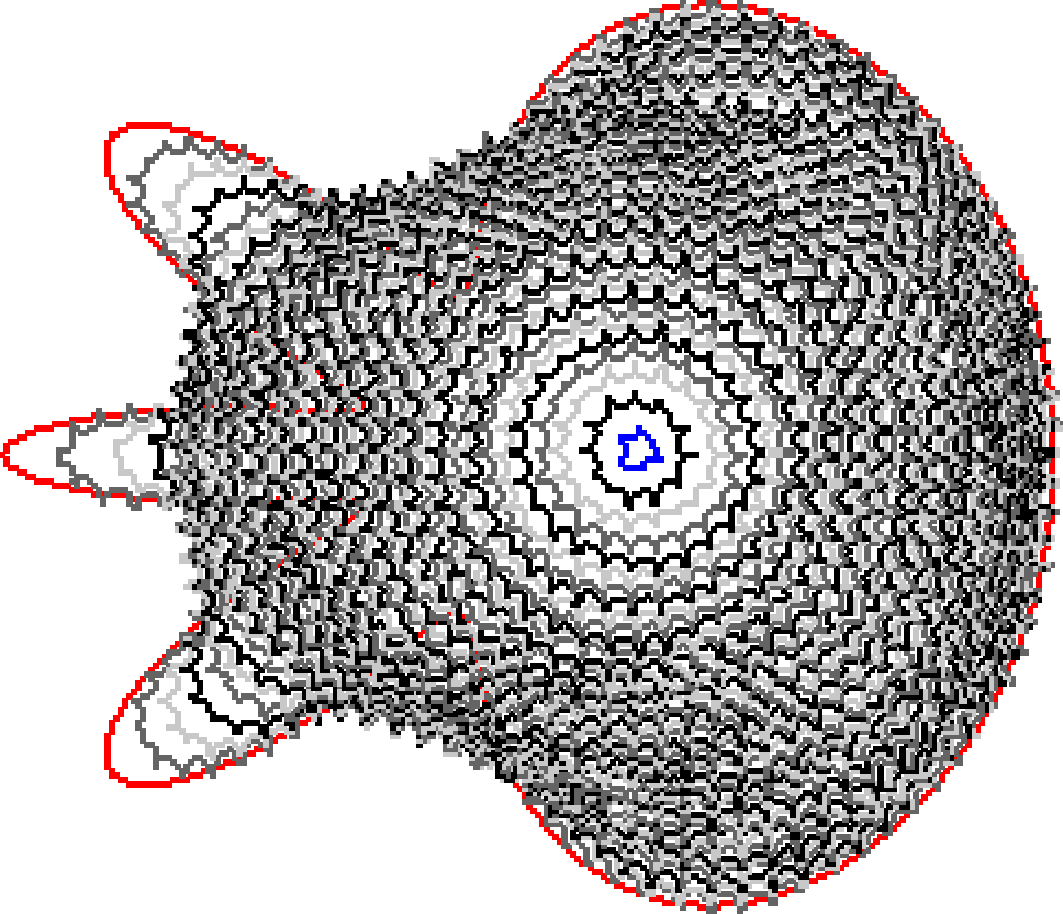
\includegraphics[scale=0.22]{figures/chapter6/level-effect/flower/improve/len_pen0/radius-5/level1/summary.pdf} &
%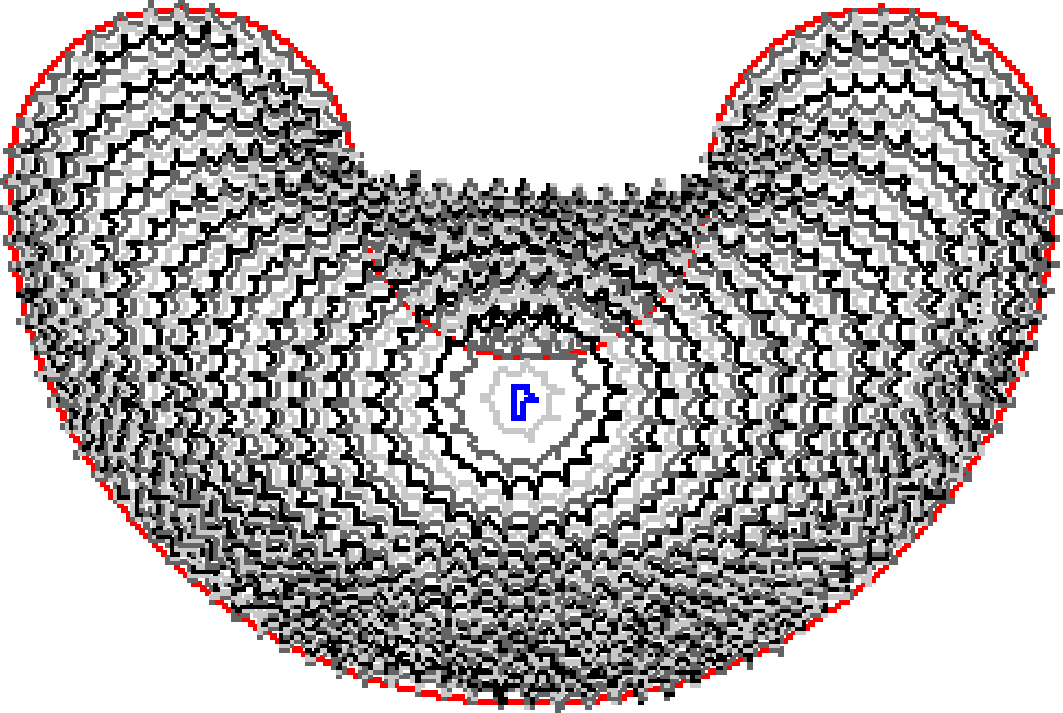
\includegraphics[scale=0.22]{figures/chapter6/level-effect/bean/improve/len_pen0/radius-5/level1/summary.pdf} \\[2em]
%$m=3$ & 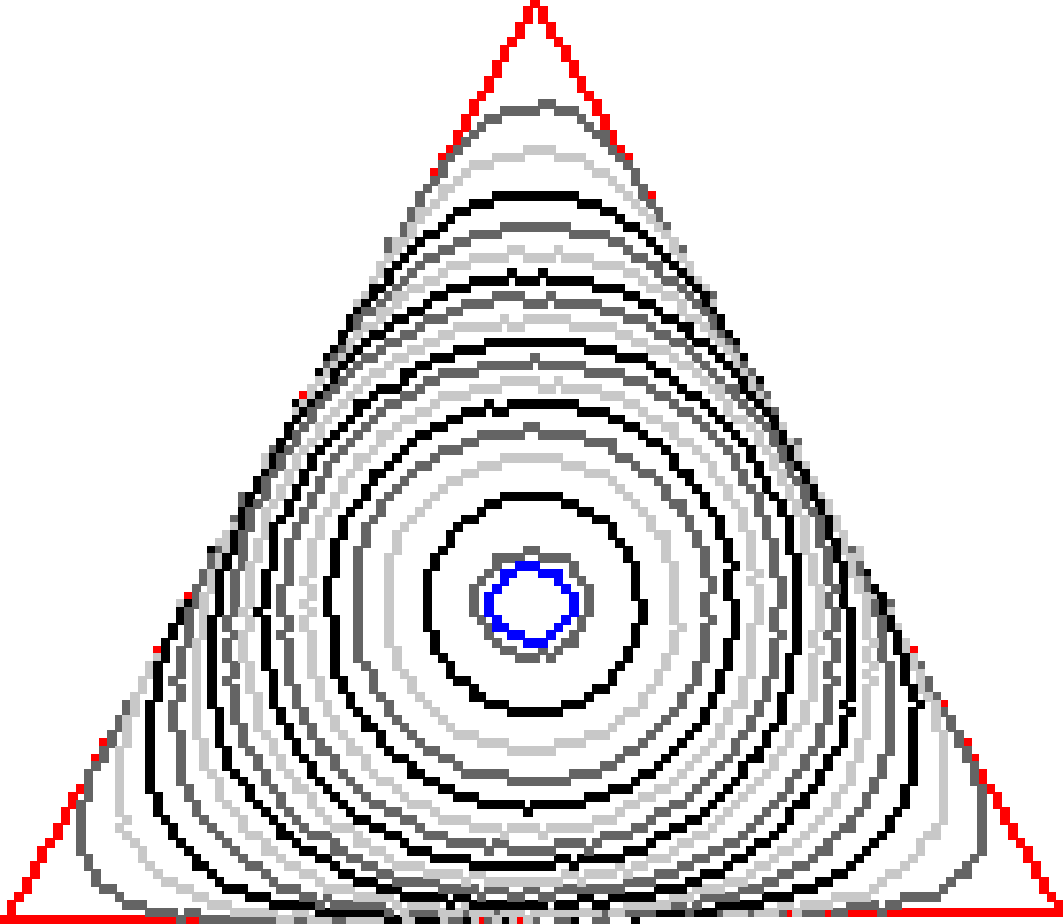
\includegraphics[scale=0.22]{figures/chapter6/level-effect/triangle/improve/len_pen0/radius-5/level3/summary.pdf} &
%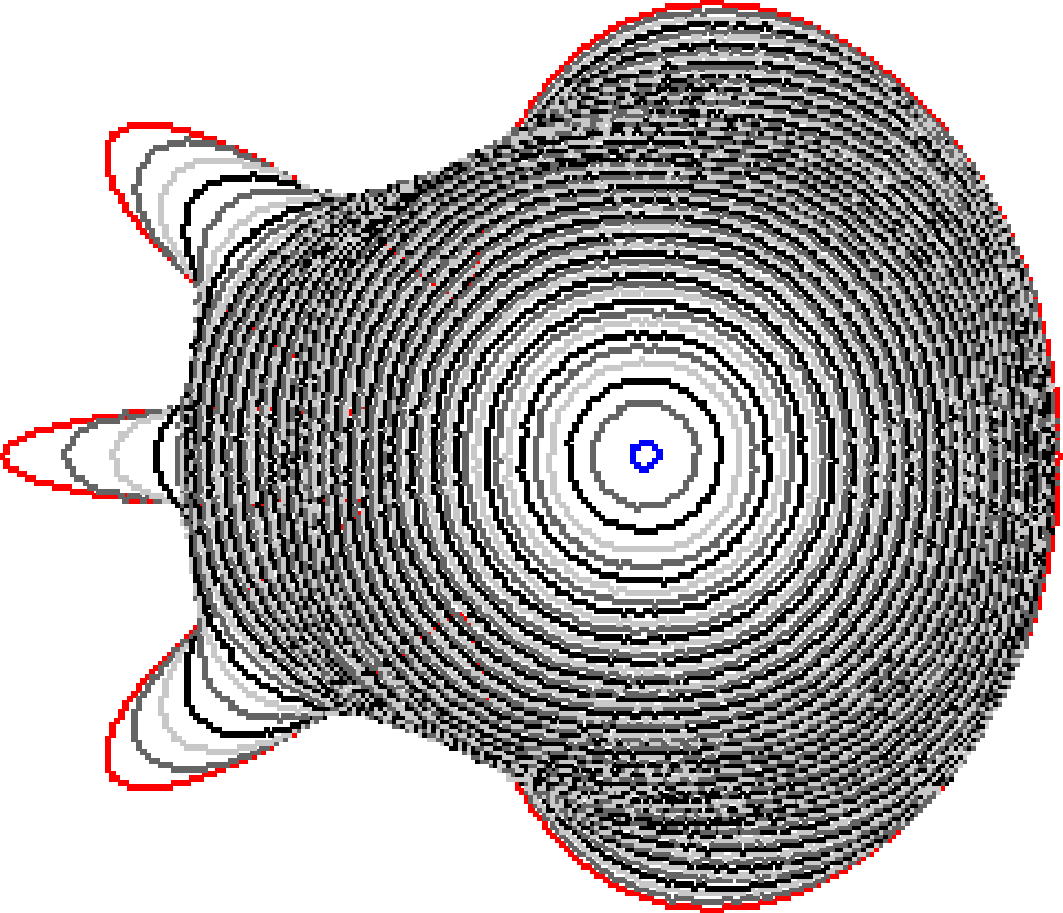
\includegraphics[scale=0.22]{figures/chapter6/level-effect/flower/improve/len_pen0/radius-5/level3/summary.pdf} &
%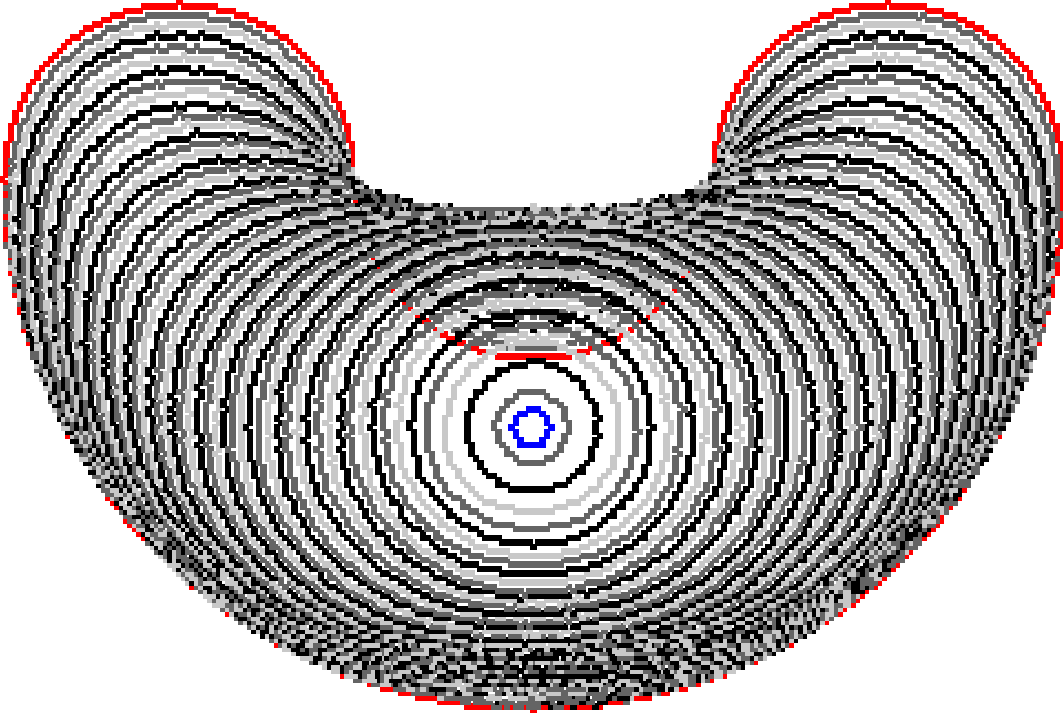
\includegraphics[scale=0.22]{figures/chapter6/level-effect/bean/improve/len_pen0/radius-5/level3/summary.pdf} \\[2em]
%$m=4$ & 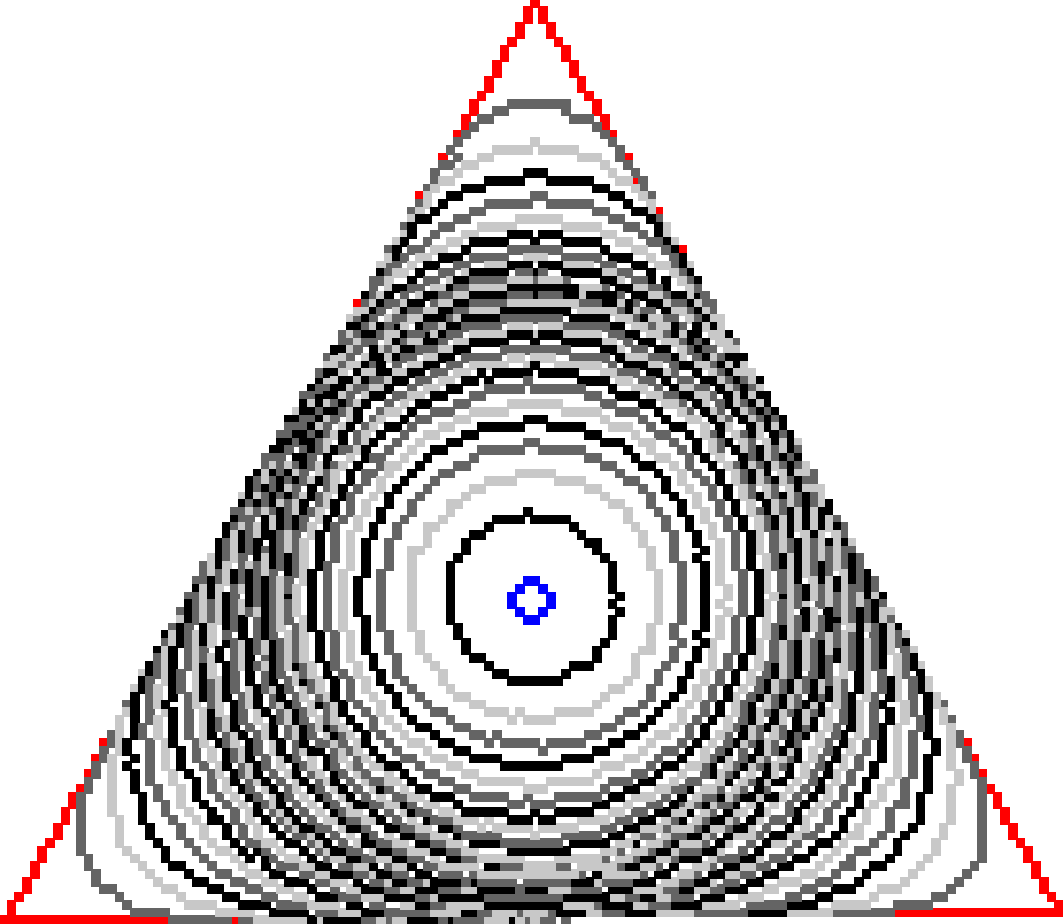
\includegraphics[scale=0.22]{figures/chapter6/level-effect/triangle/improve/len_pen0/radius-5/level4/summary.pdf} &
%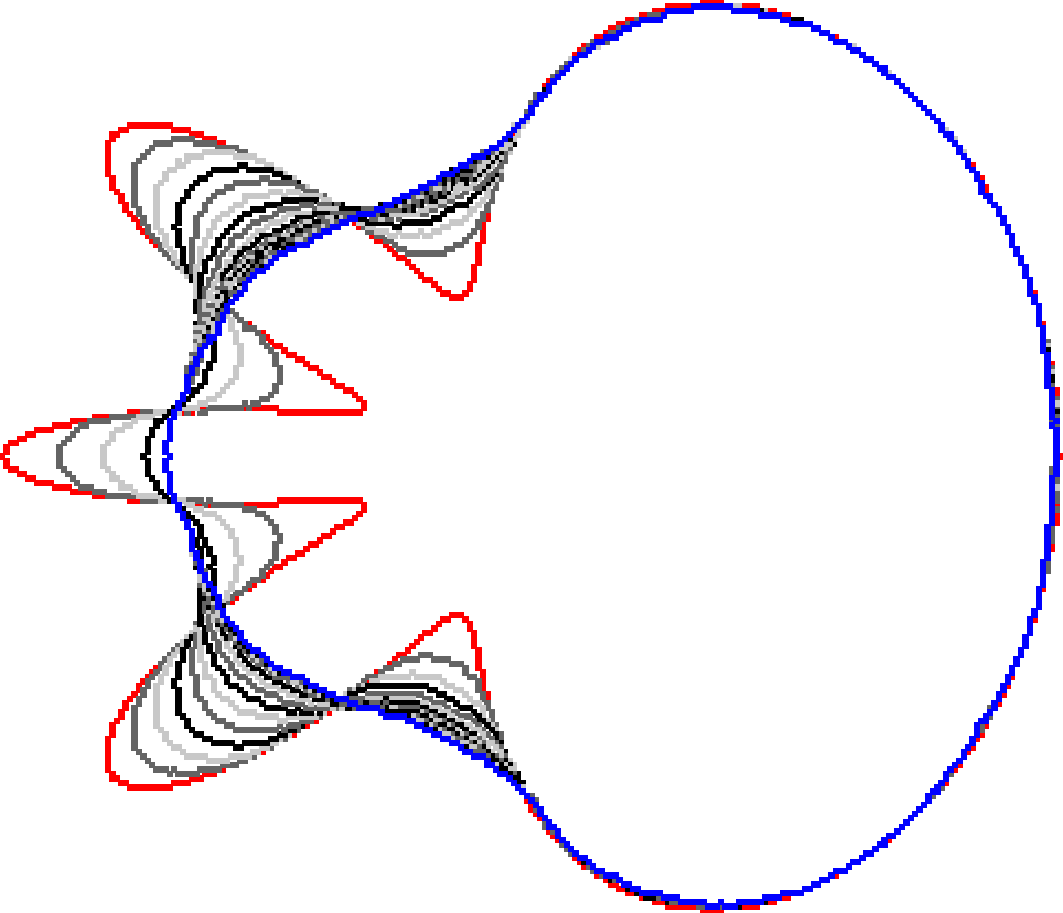
\includegraphics[scale=0.22]{figures/chapter6/level-effect/flower/improve/len_pen0/radius-5/level4/summary.pdf} &
%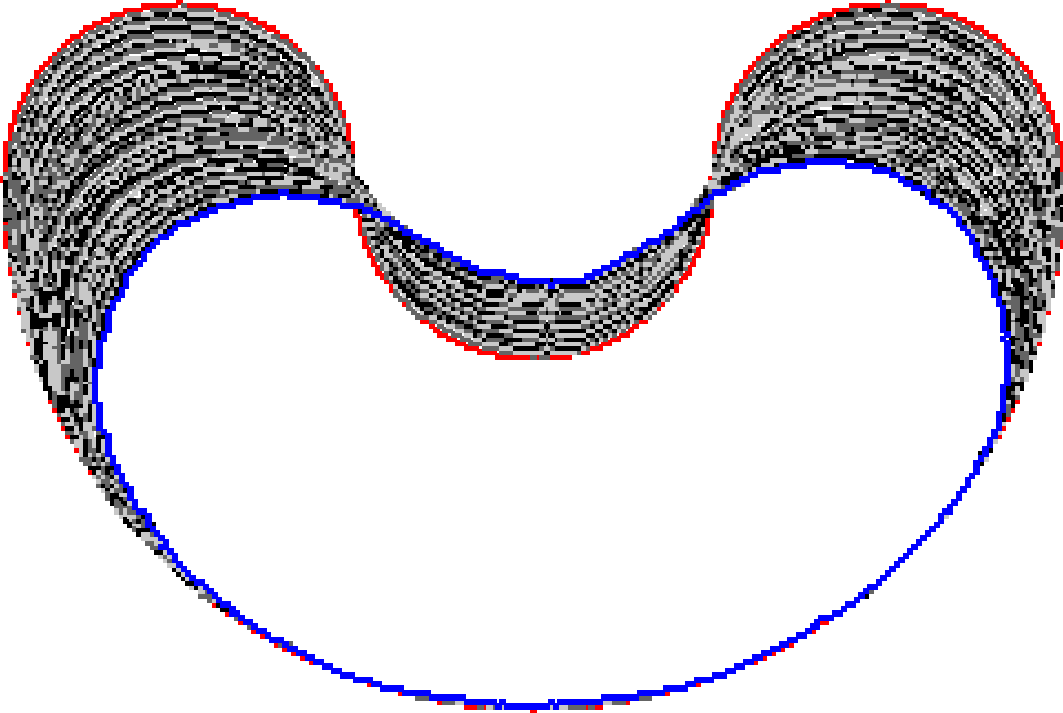
\includegraphics[scale=0.22]{figures/chapter6/level-effect/bean/improve/len_pen0/radius-5/level4/summary.pdf} \\[2em]
%$m=5$ & 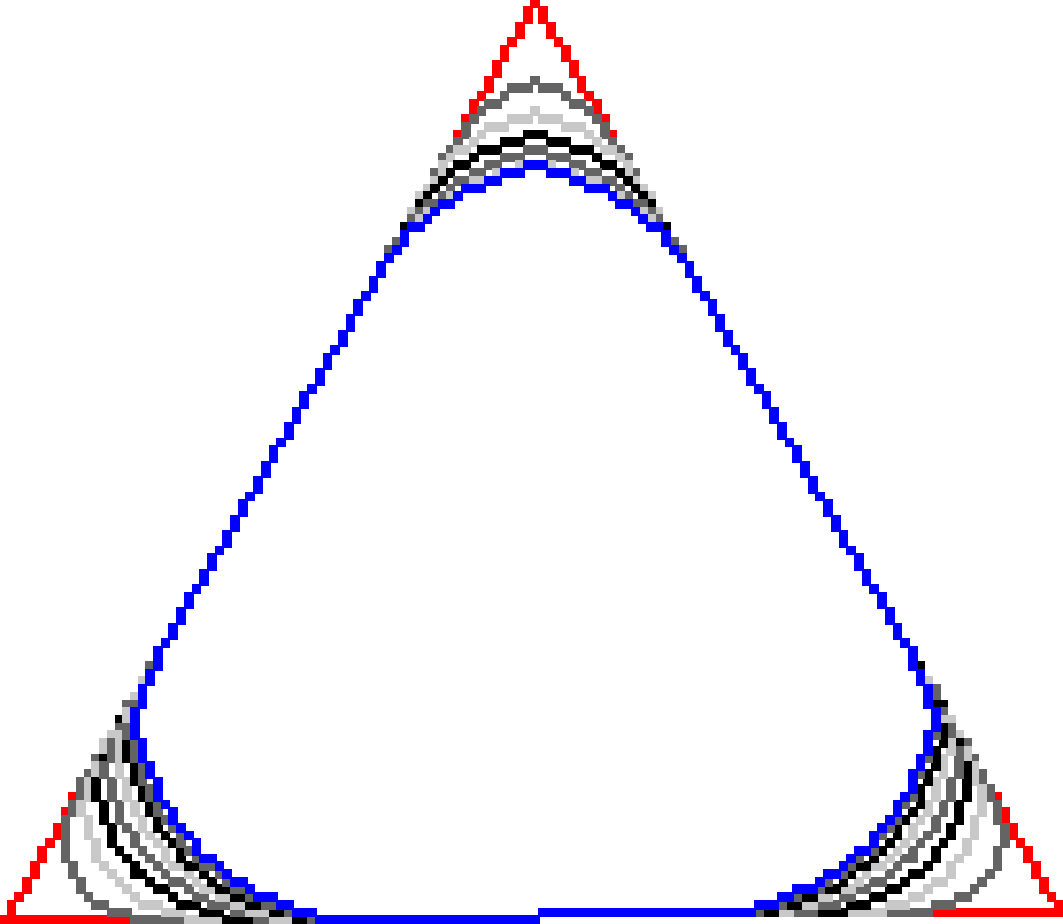
\includegraphics[scale=0.22]{figures/chapter6/level-effect/triangle/improve/len_pen0/radius-5/level5/summary.pdf} &
%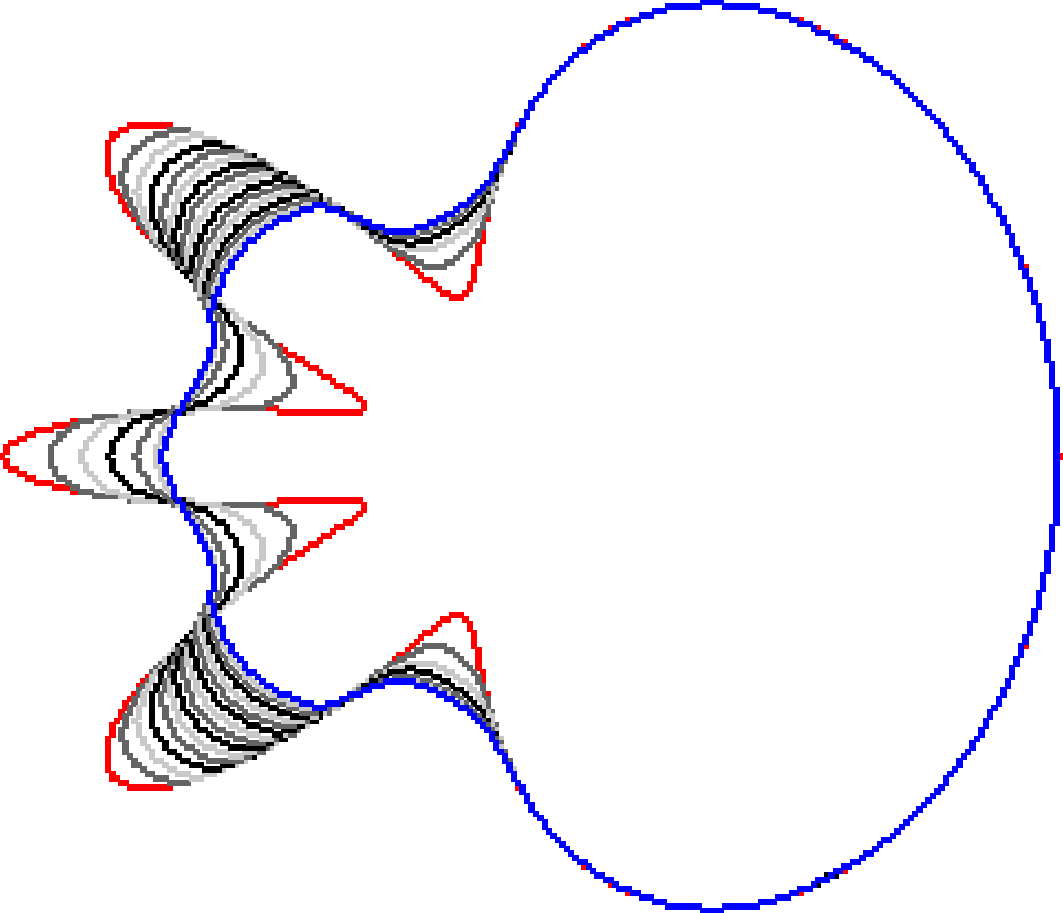
\includegraphics[scale=0.22]{figures/chapter6/level-effect/flower/improve/len_pen0/radius-5/level5/summary.pdf} &
%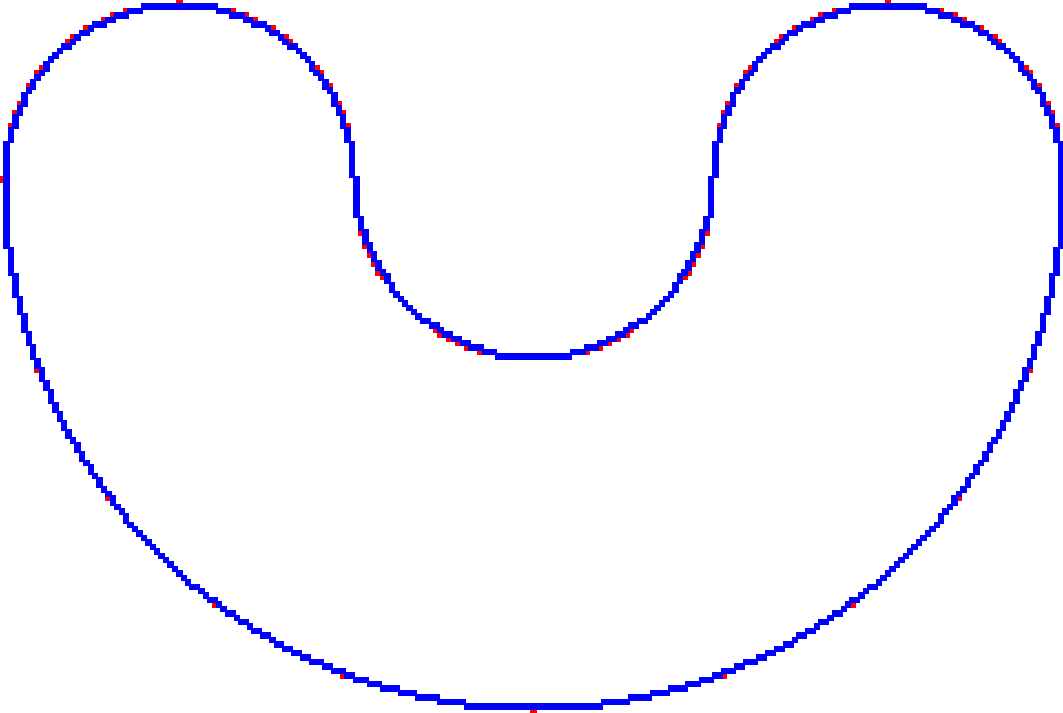
\includegraphics[scale=0.22]{figures/chapter6/level-effect/bean/improve/len_pen0/radius-5/level5/summary.pdf} \\[2em]
%\end{tabular}
%\caption{\daniel{\textbf{FlipFlow results for $\mathbf{r=5}$.}} By positioning the estimation ball on outer rings, we minimize artifacts creation. %The radius of the estimation ball used here equals to $5$ and the curves are displayed every $10$ iterations.
%}
%\label{ch6:fig:mrings-r5-evolution}
%\end{figure}
%
%
%\begin{figure}
%\center
%\begin{tabular}{p{3em}ccc}
%$m=1$ & 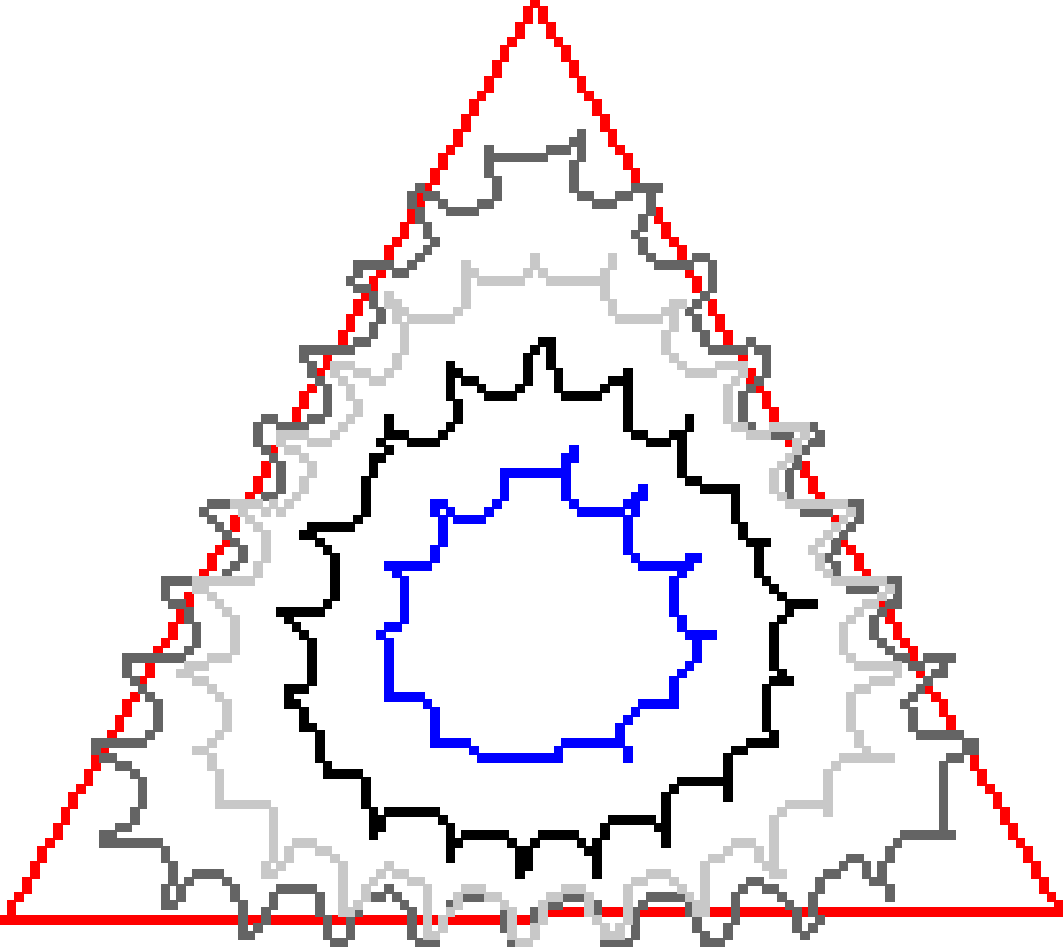
\includegraphics[scale=0.22]{figures/chapter6/level-effect/triangle/improve/len_pen0/radius-9/level1/summary.pdf} &
%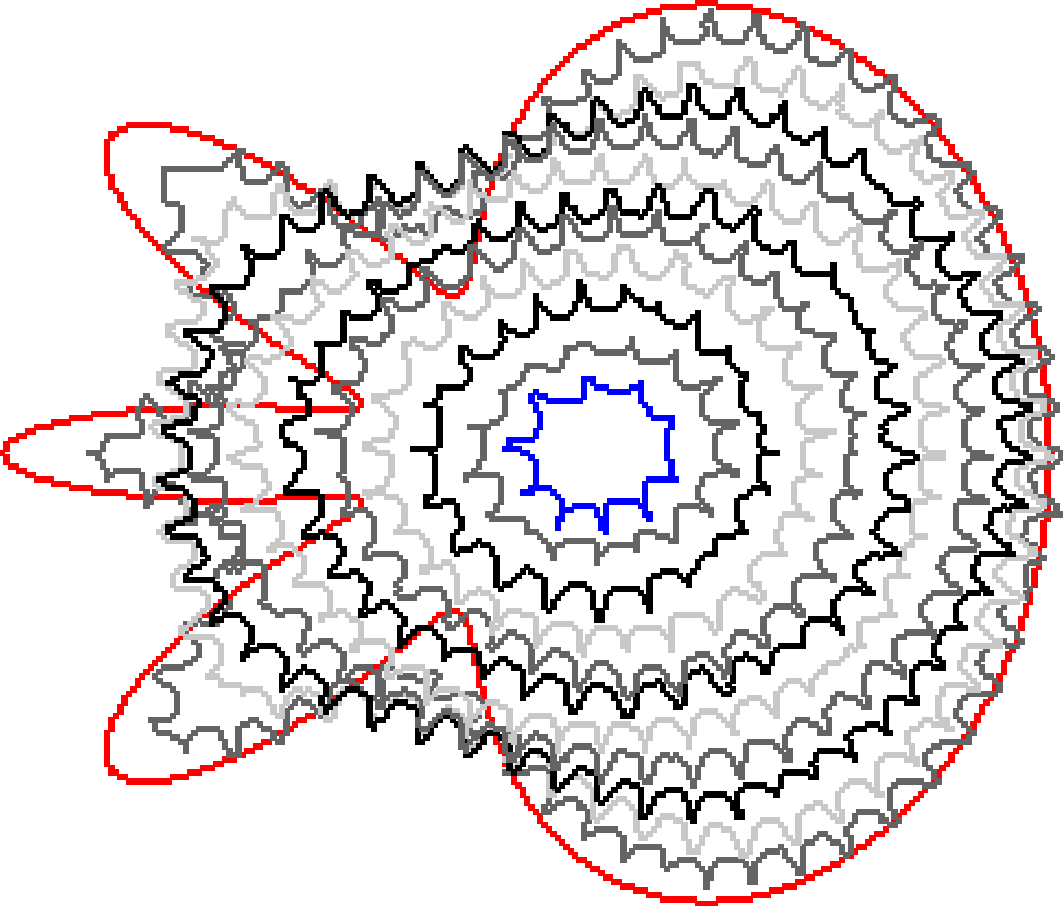
\includegraphics[scale=0.22]{figures/chapter6/level-effect/flower/improve/len_pen0/radius-9/level1/summary.pdf} &
%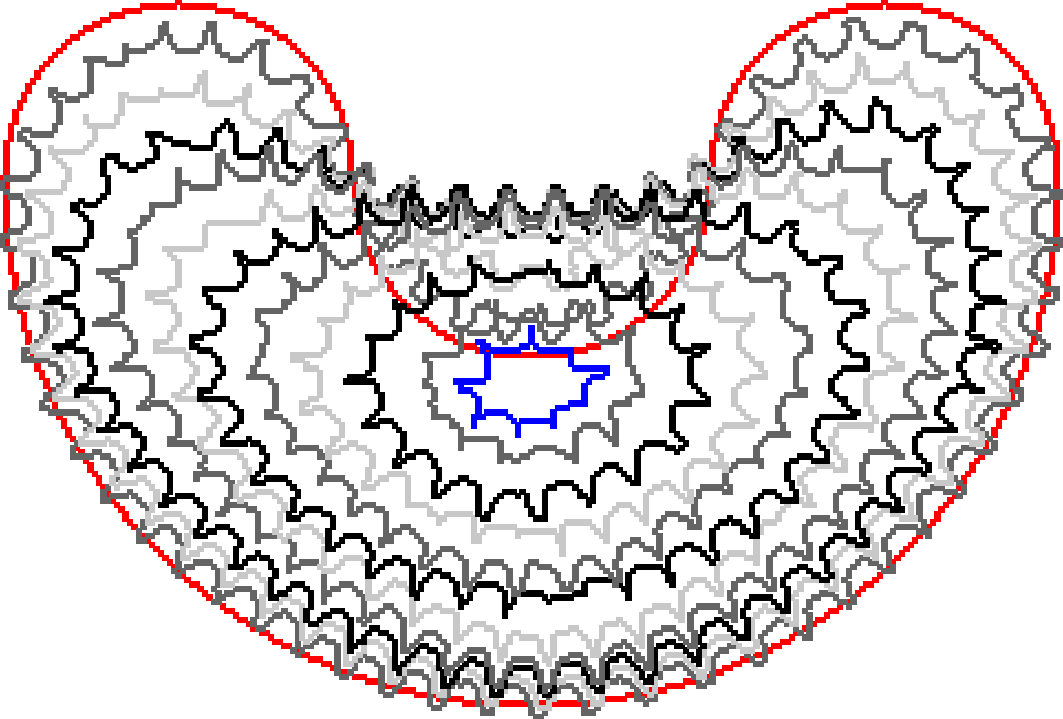
\includegraphics[scale=0.22]{figures/chapter6/level-effect/bean/improve/len_pen0/radius-9/level1/summary.pdf} \\[2em]
%$m=5$ & 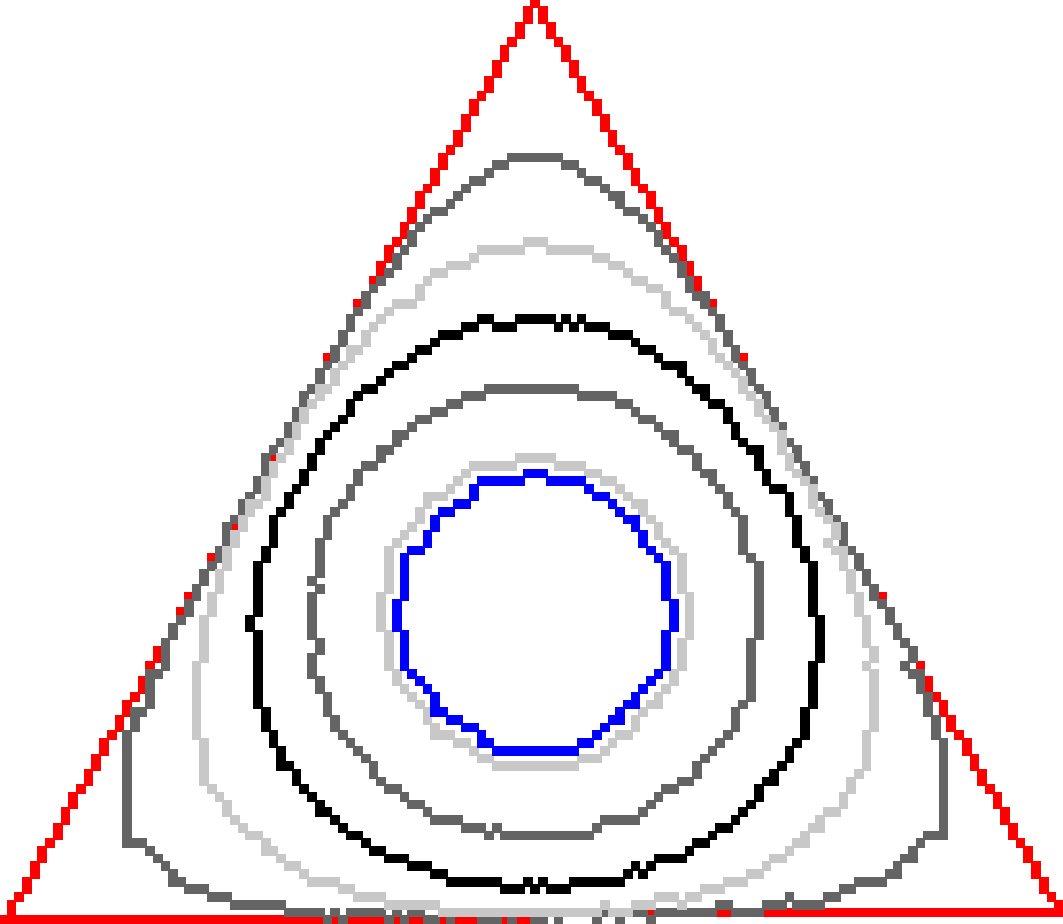
\includegraphics[scale=0.22]{figures/chapter6/level-effect/triangle/improve/len_pen0/radius-9/level5/summary.pdf} &
%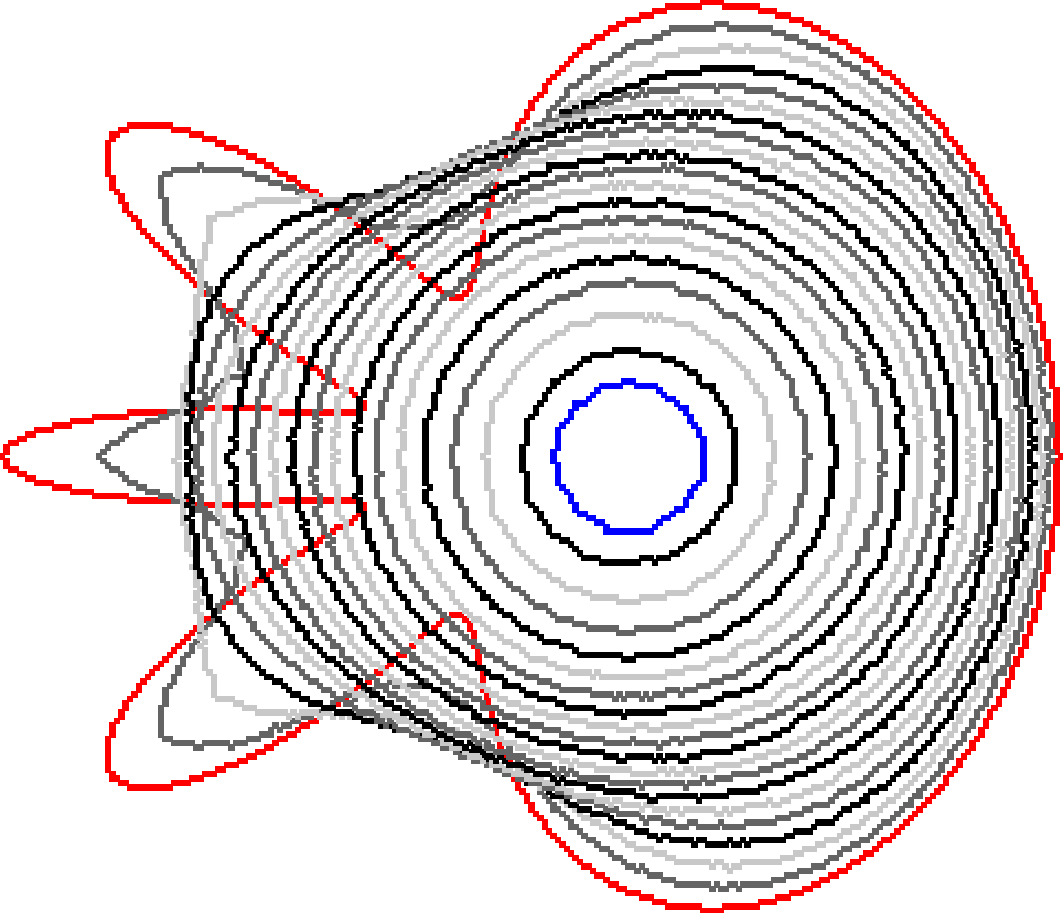
\includegraphics[scale=0.22]{figures/chapter6/level-effect/flower/improve/len_pen0/radius-9/level5/summary.pdf} &
%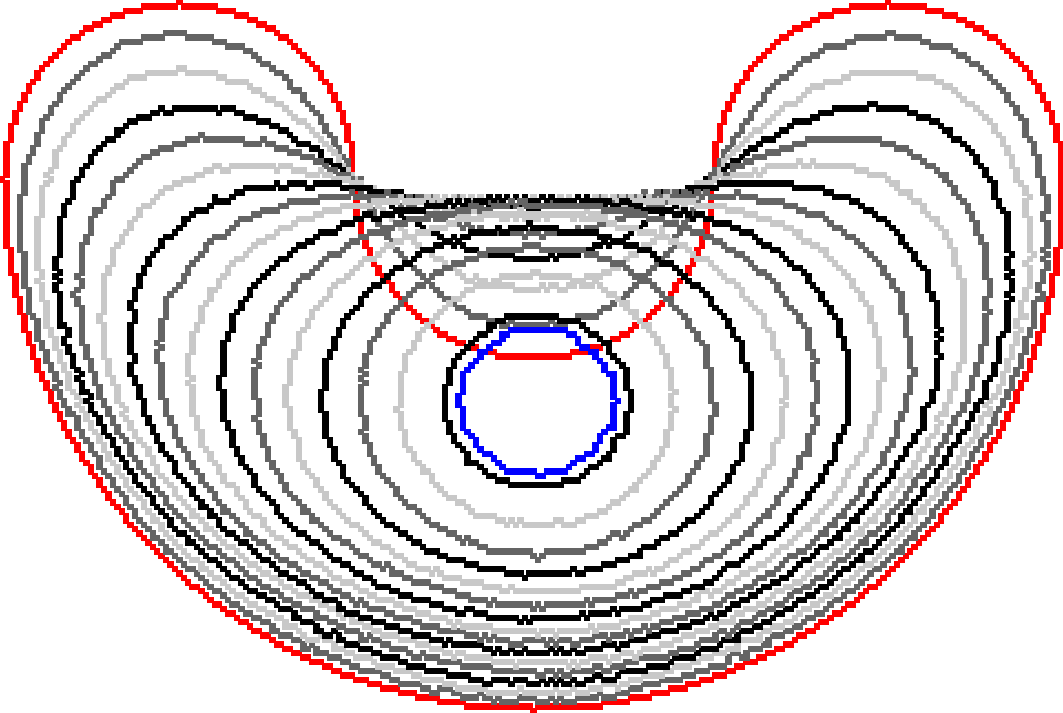
\includegraphics[scale=0.22]{figures/chapter6/level-effect/bean/improve/len_pen0/radius-9/level5/summary.pdf} \\[2em]
%$m=8$ & 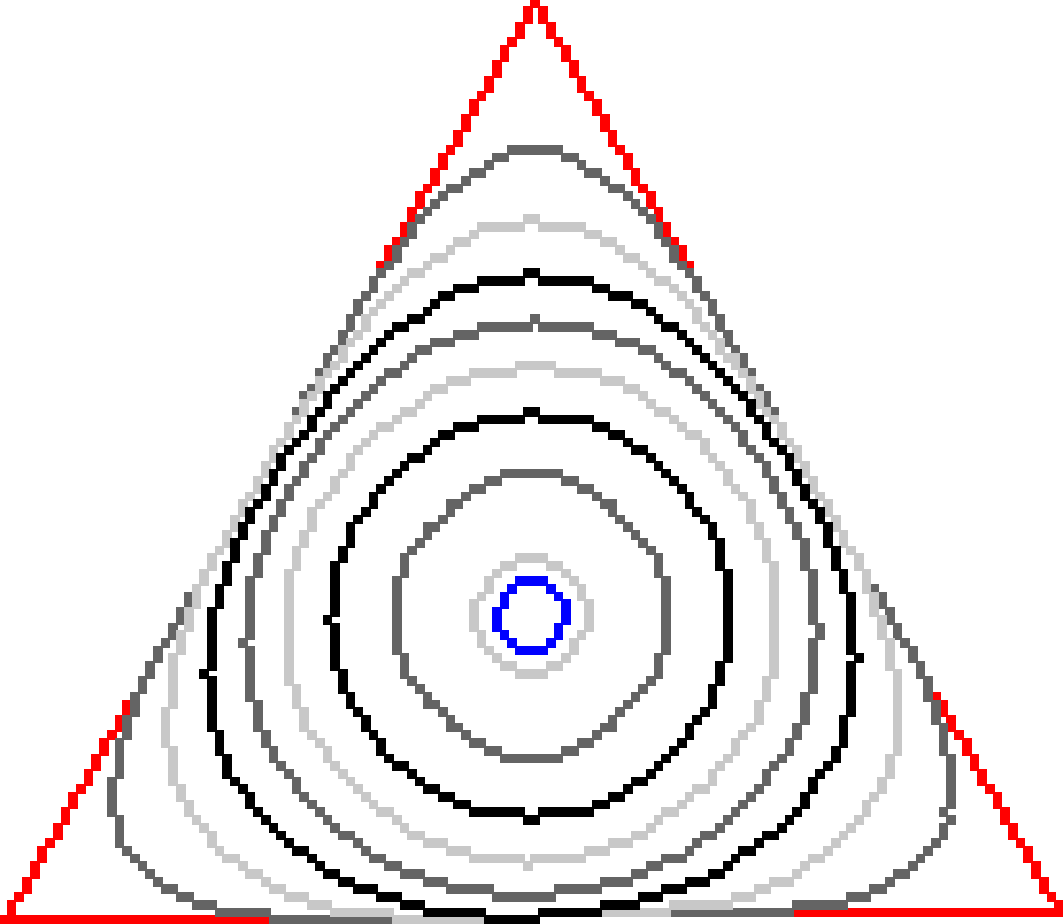
\includegraphics[scale=0.22]{figures/chapter6/level-effect/triangle/improve/len_pen0/radius-9/level8/summary.pdf} &
%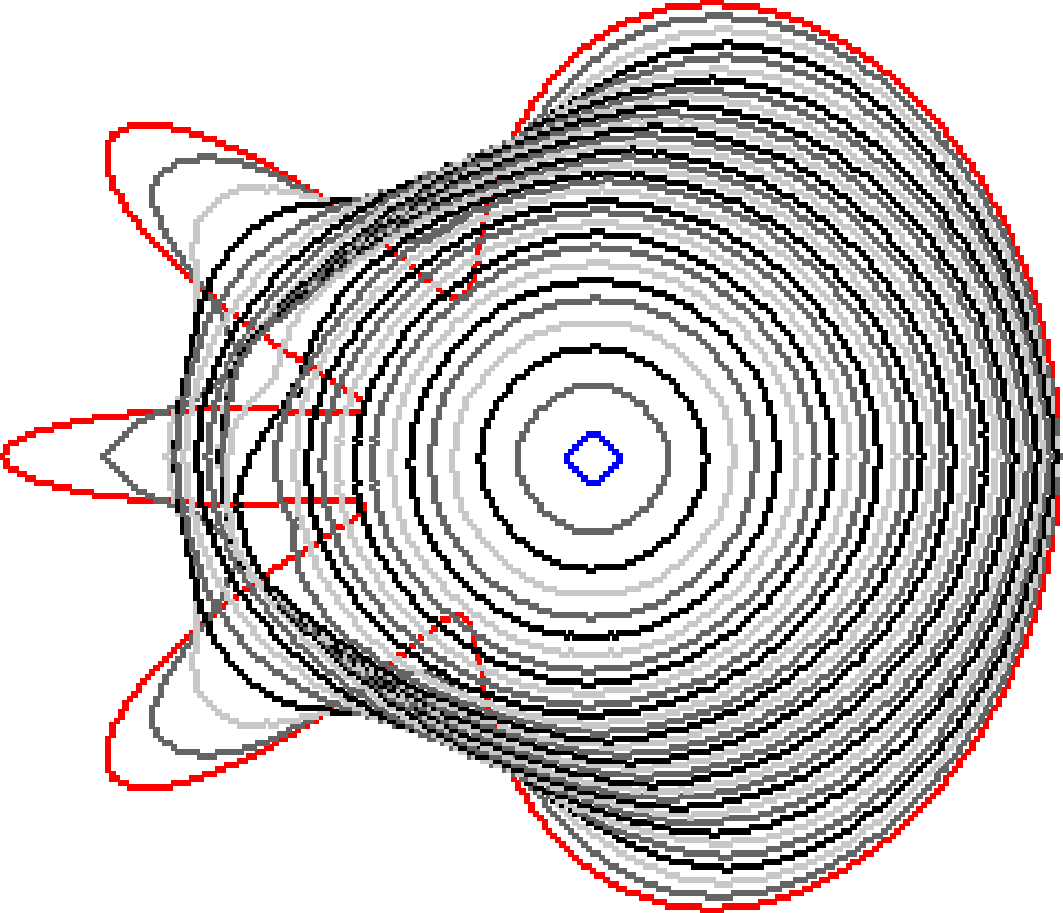
\includegraphics[scale=0.22]{figures/chapter6/level-effect/flower/improve/len_pen0/radius-9/level8/summary.pdf} &
%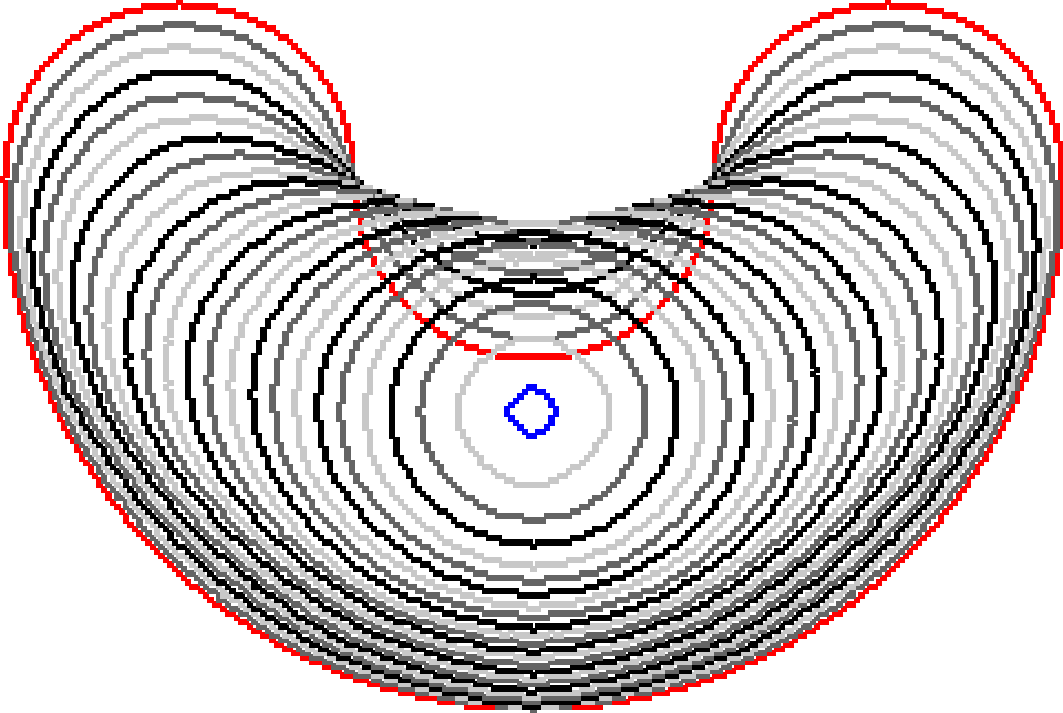
\includegraphics[scale=0.22]{figures/chapter6/level-effect/bean/improve/len_pen0/radius-9/level8/summary.pdf} \\[2em]
%$m=9$ & 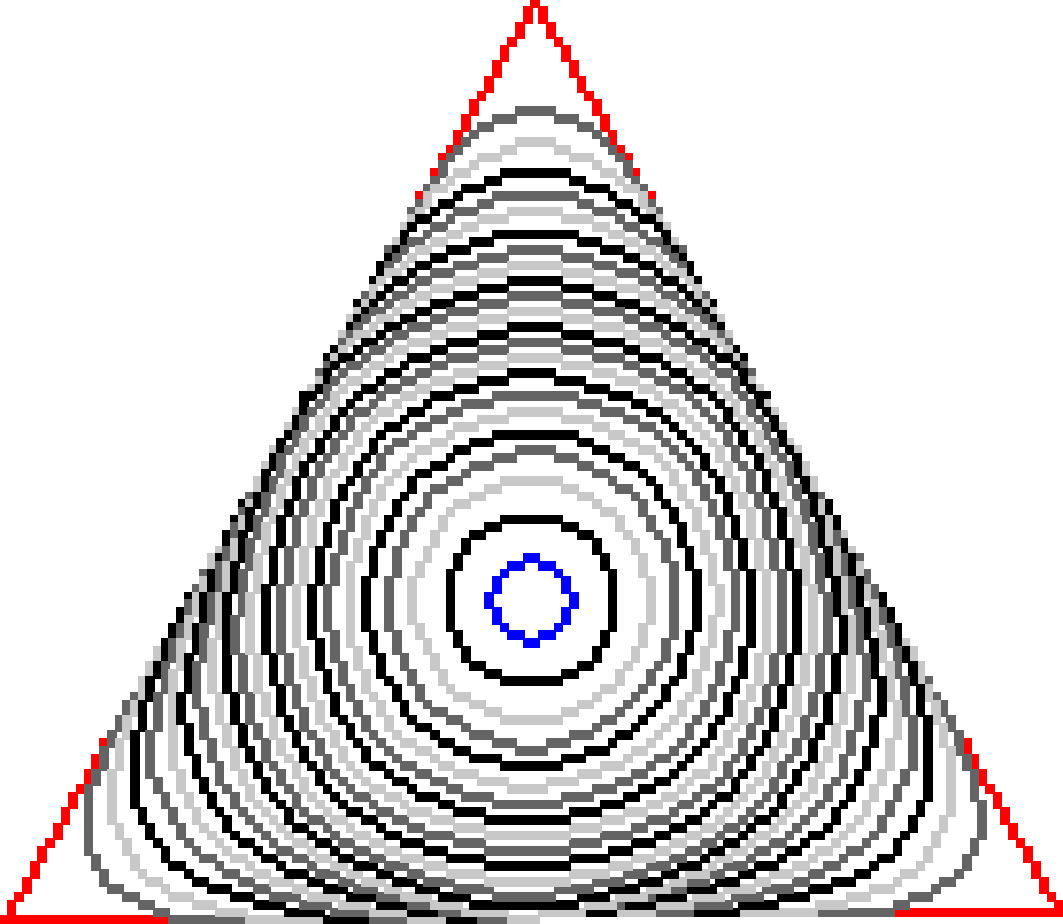
\includegraphics[scale=0.22]{figures/chapter6/level-effect/triangle/improve/len_pen0/radius-9/level9/summary.pdf} &
%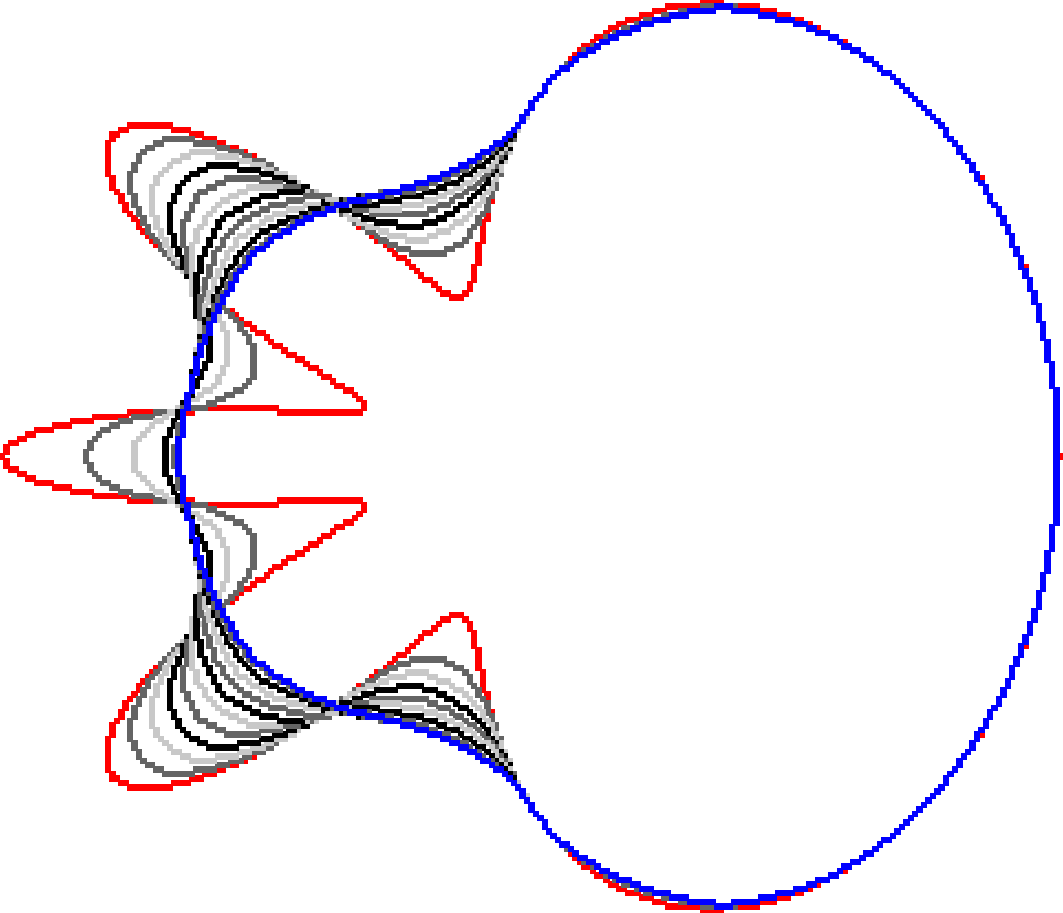
\includegraphics[scale=0.22]{figures/chapter6/level-effect/flower/improve/len_pen0/radius-9/level9/summary.pdf} &
%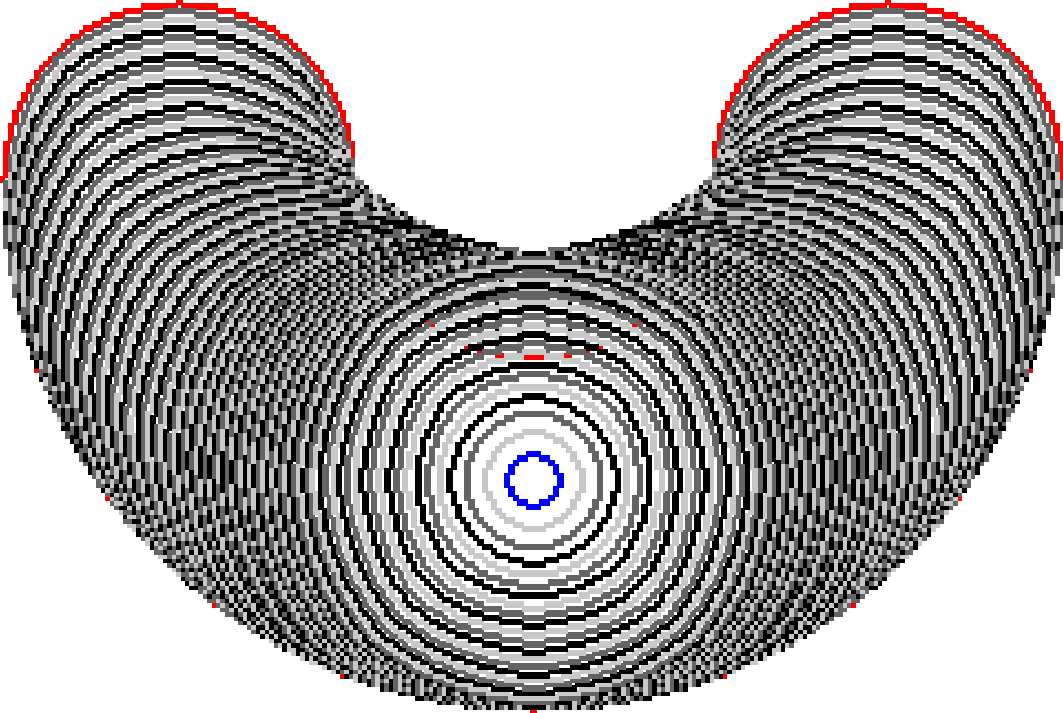
\includegraphics[scale=0.22]{figures/chapter6/level-effect/bean/improve/len_pen0/radius-9/level9/summary.pdf} \\[2em]
%\end{tabular}
%\caption{\daniel{\textbf{FlipFlow results for $\mathbf{r=9}$.}} By positioning the estimation ball on outer rings, we minimize artifacts creation. %The radius of the estimation ball used here equals to $9$ and the curves are displayed every $10$ iterations.
%}
%\label{ch6:fig:mrings-r9-evolution}
%\end{figure}



\begin{figure}
\center
\begin{tabular}{ccc}
$m=1$ & $m=4$ & $m=5$\\
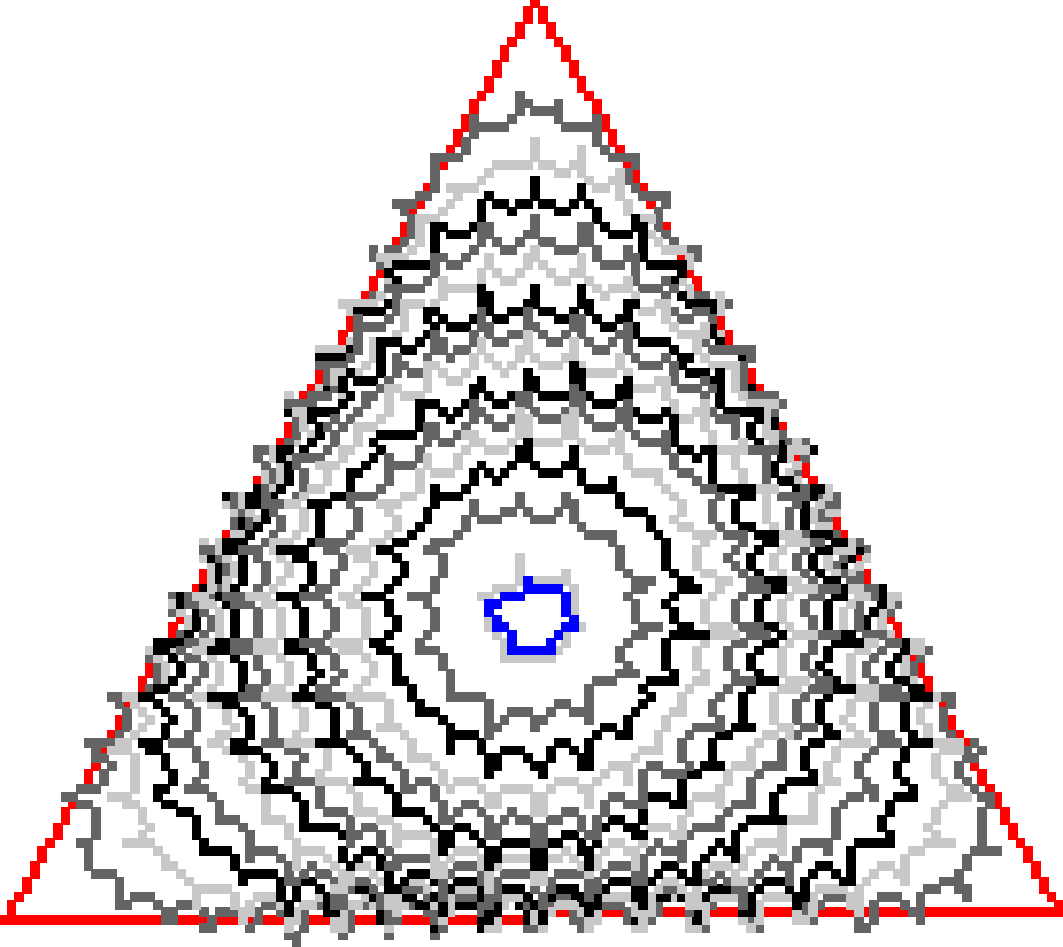
\includegraphics[scale=0.22]{figures/chapter6/level-effect/triangle/improve/len_pen0/radius-5/level1/summary.pdf} &
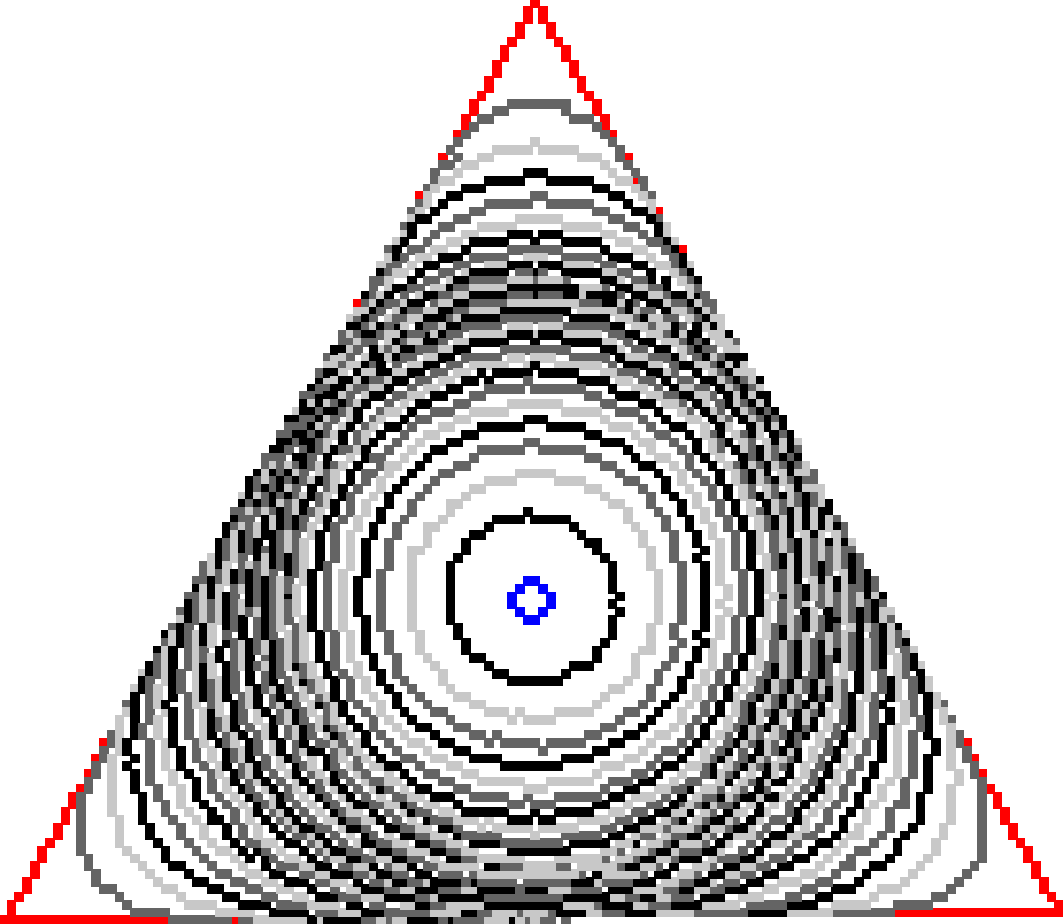
\includegraphics[scale=0.22]{figures/chapter6/level-effect/triangle/improve/len_pen0/radius-5/level4/summary.pdf} &
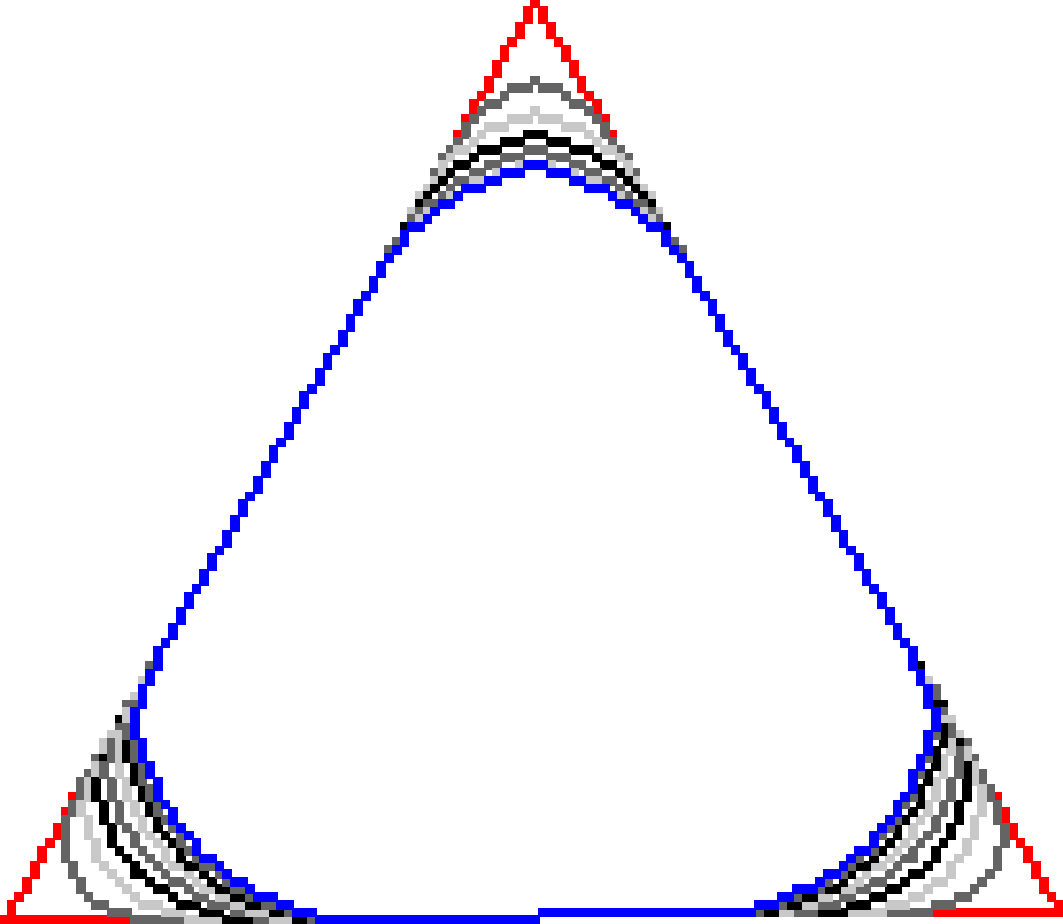
\includegraphics[scale=0.22]{figures/chapter6/level-effect/triangle/improve/len_pen0/radius-5/level5/summary.pdf}\\[2em]
\includegraphics[scale=0.22]{figures/chapter6/level-effect/flower/improve/len_pen0/radius-5/level1/summary.pdf} &
\includegraphics[scale=0.22]{figures/chapter6/level-effect/flower/improve/len_pen0/radius-5/level4/summary.pdf} &
\includegraphics[scale=0.22]{figures/chapter6/level-effect/flower/improve/len_pen0/radius-5/level5/summary.pdf} 
\end{tabular}
\caption{\daniel{\textbf{FlipFlow results for $\mathbf{r=5}$.}} By positioning the estimation ball on outer rings, we minimize artifacts creation. %The radius of the estimation ball used here equals to $5$ and the curves are displayed every $10$ iterations.
}
\label{ch6:fig:mrings-r5-evolution}
\end{figure}


\begin{figure}
\center
\begin{tabular}{ccc}
$m=1$ & $m=6$ & $m=9$\\
\includegraphics[scale=0.22]{figures/chapter6/level-effect/triangle/improve/len_pen0/radius-9/level1/summary.pdf} &
\includegraphics[scale=0.22]{figures/chapter6/level-effect/triangle/improve/len_pen0/radius-9/level6/summary.pdf} &
\includegraphics[scale=0.22]{figures/chapter6/level-effect/triangle/improve/len_pen0/radius-9/level9/summary.pdf}\\[2em]
\includegraphics[scale=0.22]{figures/chapter6/level-effect/flower/improve/len_pen0/radius-9/level1/summary.pdf} &
\includegraphics[scale=0.22]{figures/chapter6/level-effect/flower/improve/len_pen0/radius-9/level6/summary.pdf} &
\includegraphics[scale=0.22]{figures/chapter6/level-effect/flower/improve/len_pen0/radius-9/level9/summary.pdf}
\end{tabular}
\caption{\daniel{\textbf{FlipFlow results for $\mathbf{r=9}$.}} By positioning the estimation ball on outer rings, we minimize artifacts creation. %The radius of the estimation ball used here equals to $9$ and the curves are displayed every $10$ iterations.
}
\label{ch6:fig:mrings-r9-evolution}
\end{figure}




\begin{figure}
\center
\subfloat[]{
\includegraphics[scale=0.4]{figures/chapter6/level-effect/triangle/improve/len_pen0/radius-5/level1/level-effect.pdf}}%
\subfloat[]{
\includegraphics[scale=0.4]{figures/chapter6/level-effect/triangle/improve/len_pen0/radius-9/level1/level-effect.pdf}}%


\subfloat[]{
\includegraphics[scale=0.4]{figures/chapter6/level-effect/flower/improve/len_pen0/radius-5/level1/level-effect.pdf}}%
\subfloat[]{
\includegraphics[scale=0.4]{figures/chapter6/level-effect/flower/improve/len_pen0/radius-9/level1/level-effect.pdf}}%
\caption{\daniel{\textbf{Digital elastica evaluation.} We present the results of the FlipFlow model for different values of $m$. %h=0.25
In the left column, we use FlipFlow radius $5$ and in the right column we use FlipFlow radius $9$. }}
\label{ch6:fig:mrings-plots-r5-r9}
\end{figure}

\begin{figure}
\center
\subfloat[]{\includegraphics[scale=0.7]{figures/chapter6/topology-change/summary-wave.pdf}}

\subfloat[]{\includegraphics[scale=0.2]{figures/chapter6/topology-change/summary-square-holes.pdf}}
\caption{\daniel{\textbf{Evolution speed and topology changes.}} The flow evolves regions of high curvature faster, as illustrated in figure (a). Figure (b) illustrates the property of the FlipFlow algorithm to handle changes in topology.}
\label{ch6:fig:handle-topology-different-speed}
\end{figure}

\begin{figure}
\center
\begin{tabular}{cccc}
\multirow{2}{*}{Seeds} & \multirow{2}{*}{Graph cut} & $\alpha=0.5, \beta=0.0,$ & $\alpha=0.5, \beta=1.0,$ \\
& & $\gamma=0.5$ & $\gamma=0.5$\\
 	\includegraphics[scale=0.25]{figures/chapter6/segmentation/coala/mt_improve/radius_5/data_0.50/sq_0.00/length_0.50/it_50/seeds.png} & 
 	\includegraphics[scale=0.25]{figures/chapter6/segmentation/coala/mt_improve/radius_5/data_0.50/sq_0.00/length_0.50/it_50/gc-seg.png} & 
 	\includegraphics[scale=0.25]{figures/chapter6/segmentation/coala/mt_improve/radius_5/data_0.50/sq_0.00/length_0.50/it_50/corrected-seg.png} & 
 	\includegraphics[scale=0.25]{figures/chapter6/segmentation/coala/mt_improve/radius_5/data_0.50/sq_1.00/length_0.50/it_50/corrected-seg.png}
\end{tabular}	
\caption{\daniel{\textbf{FlipFlow results for segmentation}.}Given foreground (green) and background (blue) seeds at picture (a); Graph cut produces picture (b) which is used as input of the Contour Correction algorithm; in pictures (c) and (d) we display the output of Contour Correction algorithm with and without squared curvature regularization. }
\label{ch6:fig:segmentation}
\end{figure}

The QPBOP method leaves many pixels unlabeled for $m=0$, \daniel{but in some occasions, the ratio of unlabeled pixels decreases as we take values of $m$ closer to $r$}. In this section, we argue that by evaluating the estimation ball along outer rings we obtain smoother evolutions by focusing the optimization process only on regions of high squared curvature value.

In~\cref{ch6:fig:mrings-r5-evolution,ch6:fig:mrings-r9-evolution} we evaluate several flows for different energies $E_{(\vec{\theta},m)}^{flip}$. As expected, the number of artifacts decrease as the value of $m$ increases, while the process still tends to shrink the shape to a single point, resembling the \daniel{curve shortening flow discussed in~\cref{ch3:sec:curvature-curve-shortening-flow}}. 

We confirm the stability of the model by looking at the plots of the digital elastica energy values for the produced shapes. Moreover, the produced flow has no difficulties in handling changes on topology, and it presents different speeds for regions with low and high curvature values, as illustrated in~\cref{ch6:fig:handle-topology-different-speed}.

The computation of estimation balls at outer rings raises the question about its validity as a curvature estimator. In fact, one can estimate the curvature using outer balls (see~\cref{app:curvature-and-distant-disks}), but we were not able to prove its multigrid convergence. However, this relation suggests that curvature information is at least qualitatively present in the outer balls computation, and this computation is preferred, as it is easier to optimize accordingly to the experiments illustrated in~\cref{ch6:fig:mrings-r5-evolution,ch6:fig:mrings-r9-evolution,ch6:fig:unlabeled-versus-iterations,ch6:fig:mrings-plots-r5-r9}.




\section{Data term and image segmentation}
\label{ch6:sec:data-term-image-segmentation}

We present an application of the FlipFlow algorithm to supervised image segmentation. The FlipFlow acts as a contour correction method. Here we use a data fidelity term in order to characterize the object of interest. Given foreground and background seeds selected by the user, we derive mixed Gaussian distributions of color intensities $H_f$,$H_b$, and we define the data fidelity term as the cross-entropy, i.e.
\begin{align}
  g(x_{w(p)}) = -x_{w(p)}\log{H_f(p)} - (1-x_{w(p)})\log{H_b(p)}
  \label{eq:data-fidelity}
\end{align}	
%
We use the FlipFlow algorithm to regularize an initial contour output by some segmentation algorithm or delineated by the user. In this application, the data term of the FlipFlow
is set to the data fidelity term~\cref{eq:data-fidelity}.
	
\begin{algorithm}[]
 \SetKwData{It}{k}
 \SetKwData{MIt}{maxIt}
 \SetKwData{Tol}{tolerance}
 \SetKwData{Delta}{delta}
 \SetKwInOut{Input}{input}\SetKwInOut{Output}{output}
 \SetKwComment{comment}{//}{}
 
 \Input{An image $I$; seeds mask $M$; the estimation ball radius $r$; parameter vector $\vec{\theta}=(\alpha, \beta)$; data term weight $(\gamma)$ ; initial dilation $d$; stop condition value \Tol; the maximum number of iterations \MIt;}
 \BlankLine

 $\Ds \longleftarrow$ Graph cut($I,M$)\;
 $\Ds^{(0)} \longleftarrow $ dilate($\Ds$,$d$)\; 
 \Delta $\longleftarrow +\infty$\;
 $k \longleftarrow 0$\;
 \While{ \It $<$ \MIt \bf{and} \Delta $>$ \Tol  }{ 	
 
 	\comment{Shrink mode}
	\If{ \It is even }{	 
	 	$x^{(k-1)} \longleftarrow \displaystyle \argmin_{X^{(k-1)}} E_{(\vec{\theta},m)}^{flip}(\Ds^{(k-1)},1-X^{(k-1)}) + \gamma g(X^{(k-1)})$\; 	
 		$\Ds^{(k)} \longleftarrow F^{(k-1)} + x^{(k-1)}$\;
 	}
	\comment{Expansion mode} 	
 	\Else{	
	 	$\overline{x}^{(k-1)} \longleftarrow \displaystyle \argmin_{\overline{X}^{(k-1)}} E_{(\vec{\theta},m)}^{flip}(\Ds^{(k-1)},1-\overline{X}^{(k-1)}) + \gamma g(\overline{X}^{(k-1)})$\;
 		$\Ds^{(k)} \longleftarrow \overline{ \overline{F}^{(k-1)} + \overline{x}^{(k-1)}}$\; 	
 	}
 

 	\Delta $\longleftarrow |\Ds^{(k)} \setminus \Ds^{(k+1)}|$\;

	\It $\longleftarrow$ \It $+1$\;
	
 }
 \caption{FlipFlow algorithm for segmentation.}
  \label{ch6:alg:contour-correction} 
\end{algorithm}	

The algorithm can be initialized by a collection of compact sets, or with the result of a third-party segmentation algorithm, as Graph cut~\cite{boykov01graphcut}. We include an additional parameter $d$ that dilates the initial sets using a square of side one before executing the flow.

An illustration of the application of the FlipFlow model in image segmentation is presented in~\cref{ch6:fig:segmentation}. We present a more exhaustive list of experiments and comparisons with other methods in~\cref{chapter:results-analysis}.


\section{Conclusion}
\label{ch6:sec:conclusion}
\daniel{
We proposed the FlipFlow algorithm, an evolution process based on the minimization of a second-order non-submodular energy that produces shapes of decreasing digital elastica until a certain inflexion point. We point out the submodularization effect of evaluating the FlipFlow model at outer $m$-rings and we observed that the model evolves the shapes in a similar fashion to the curve-shortening flow for an appropriate choice of parameters. 

The FlipFlow operates in two distinct modes: the shrink and the expansion modes. They are responsible for the treatment of convexities and concavities regions, respectively. The model handles changes in topology and can be extended to include extra terms as data regularization term. In particular, we described an application of the FlipFlow model to image segmentation.

It is remarkable that curvature regularization is achieved by evaluating the estimation disks at outer rings. It is also surprising the fact that we are using a quite non-standard operation of taking the solution complement. We have developed an heuristic reasoning to explain the latter and we argue in~\cref{app:curvature-and-distant-disks} that curvature can still be measured evaluating disks at outer rings. Nonetheless, we may have taken an unnecessary tortuous path and missed the fundamental concept behind it. In the next chapter we identify the key concept behind the FlipFlow model to define a variant of this algorithm which is easier to implement.
}

%We presented the FlipFlow model in~\cref{ch6:sec:flipflow-model}, an evolution process that produces shapes of decreasing digital elastica until a certain inflexion point.~\cref{ch6:alg:evolution-model} operates in two distinct modes: the shrink and the expansion modes. They are responsible for the treatment of convexities and concavities regions, respectively. 
%
%~\cref{ch6:sec:optimization-method} briefly describes some properties of QPBO method and its variants used to solve the quadratic binary problem that appears at every iteration of ~\cref{ch6:alg:evolution-model}. In~\cref{ch6:sec:evaluation-across-rings} we point out the submodularization effect of evaluating the FlipFlow model at outer $m$-rings. For larger values of $m$, all pixels are labeled by QPBOP. Finally, we extended~\cref{ch6:alg:evolution-model} in order to include a data term regularization and do image segmentation using~\cref{ch6:alg:contour-correction}.
%
%In the next chapter we identify the key concept behind the FlipFlow model to define a variant of this algorithm which is easier to implement.